\documentclass[
	12pt,
	oneside,
	a4paper,
	chapter=TITLE,
	section=TITLE,
	english,
	brazilian
]{abntex2}

% =============================================================================
% preambulo.tex - Configuracoes Tipograficas e Pacotes (Conforme ABNT NBR 14724)
% =============================================================================

\usepackage{cmap}
\usepackage[T1]{fontenc}
\usepackage[utf8]{inputenc}

% Margens estritas da ABNT NBR 14724 (formato anverso / digital)
% Superior: 3 cm (cabecalho a 2 cm com headsep=10mm)
% Esquerda: 3 cm
% Inferior: 2 cm
% Direita:  2 cm (numero a 2 cm da borda direita)
\usepackage[
    a4paper,
    top=30mm,
    bottom=20mm,
    left=30mm,
    right=20mm,
    headheight=15pt,
    headsep=10mm,
    footskip=10mm
]{geometry}

% Tipografia padronizada Times New Roman (NBR 14724 item 5.1)
\usepackage{newtxtext}
\usepackage{newtxmath}
\usepackage[scaled=0.88]{inconsolata}

\usepackage{lastpage}
\usepackage{indentfirst}
\usepackage{microtype}
\usepackage{graphicx}
\usepackage{subcaption}
\usepackage{booktabs}
\usepackage{multirow}
\usepackage{makecell}

% Matematica avancada
\usepackage{mathtools}
\usepackage{bm}

% Unidades do SI (configuradas para o padrao brasileiro / ABNT)
\usepackage{siunitx}
\sisetup{
    output-decimal-marker={,},
    group-separator={.},
    inter-unit-product=\ensuremath{{\cdot}}
}
\DeclareSIUnit\calorie{cal}
\DeclareSIUnit\molar{mol}
\DeclareSIUnit\litre{L}

% Graficos vetoriais de alta precisao com TikZ e PGFPlots
\usepackage{tikz}
\usepackage{pgfplots}
\pgfplotsset{compat=1.18}
\usetikzlibrary{shapes.geometric,arrows.meta,positioning,calc,fit,patterns}

% Cores para codigos e diagramas
\usepackage[dvipsnames]{xcolor}

% Formatacao profissional de codigo-fonte (listings)
\usepackage{listings}
\renewcommand{\lstlistingname}{Código}
\renewcommand{\lstlistlistingname}{Lista de Códigos}

\lstdefinestyle{pythonstyle}{
    language=Python,
    basicstyle=\ttfamily\footnotesize,
    columns=flexible,
    keepspaces=true,
    keywordstyle=\color{NavyBlue}\bfseries,
    commentstyle=\color{ForestGreen}\itshape,
    stringstyle=\color{BrickRed},
    numberstyle=\tiny\color{gray},
    numbers=left,
    numbersep=8pt,
    frame=single,
    framerule=0.5pt,
    rulecolor=\color{gray!30},
    backgroundcolor=\color{gray!4},
    breaklines=true,
    breakatwhitespace=true,
    showstringspaces=false,
    captionpos=b,
    tabsize=4,
    xleftmargin=12pt,
    framexleftmargin=12pt
}
\lstset{style=pythonstyle}

% Citacoes no padrao ABNT (carrega hyperref internamente)
\usepackage[alf]{abntex2cite}

% Configuracao de links e metadados no PDF
\makeatletter
\hypersetup{
    pdftitle={\@title},
    pdfauthor={Gabriel Marques de Andrade; Elilton Rodrigues Edwards},
    pdfsubject={Relatório Técnico-Científico PROIC/FAPESB/CNPq 34/2026},
    pdfcreator={LaTeX with abnTeX2},
    colorlinks=true,
    linkcolor=NavyBlue,
    citecolor=NavyBlue,
    urlcolor=NavyBlue
}
\makeatother

% Cleveref para referencias cruzadas em portugues
\usepackage[nameinlink,brazilian]{cleveref}
\crefname{equation}{Eq.}{Eqs.}
\crefname{figure}{Figura}{Figuras}
\crefname{table}{Tabela}{Tabelas}
\crefname{chapter}{Capítulo}{Capítulos}
\crefname{section}{Seção}{Seções}
\crefname{subsection}{Subseção}{Subseções}
\crefname{lstlisting}{Código}{Códigos}

% Padronizacao tipografica dos titulos de capitulos e secoes (NBR 6024 e NBR 14724)
\renewcommand{\ABNTEXchapterfont}{\normalfont\bfseries}
\renewcommand{\ABNTEXchapterfontsize}{\Large}
\renewcommand{\ABNTEXsectionfont}{\normalfont\bfseries}
\renewcommand{\ABNTEXsectionfontsize}{\large}
\renewcommand{\ABNTEXsubsectionfont}{\normalfont\bfseries}
\renewcommand{\ABNTEXsubsectionfontsize}{\normalsize}
\renewcommand{\ABNTEXsubsubsectionfont}{\normalfont\itshape}
\renewcommand{\ABNTEXsubsubsectionfontsize}{\normalsize}
\renewcommand{\ABNTEXsubsubsubsectionfont}{\normalfont}
\renewcommand{\ABNTEXsubsubsubsectionfontsize}{\normalsize}

% Parametrizacao de paragrafo e espacamento ABNT NBR 14724
\setlength{\parindent}{1.25cm}
\setlength{\parskip}{0pt}

% Formatacao de legendas e fontes (ABNT NBR 14724 itens 5.8 e 5.9: fonte menor 10pt)
\captiondelim{ -- }
\captionnamefont{\footnotesize\bfseries}
\captiontitlefont{\footnotesize}

% Estilo de pagina textual ABNT: numero no canto superior direito, sem cabecalho
\makepagestyle{abnttextual}
\makeevenhead{abnttextual}{}{}{\footnotesize\thepage}
\makeoddhead{abnttextual}{}{}{\footnotesize\thepage}
\makeevenfoot{abnttextual}{}{}{}
\makeoddfoot{abnttextual}{}{}{}

% Redefinicao da Capa no padrao institucional UESC / ABNT NBR 14724
\renewcommand{\imprimircapa}{%
  \begin{capa}%
    \center
    {\ABNTEXchapterfont\bfseries\normalsize\MakeTextUppercase{\imprimirinstituicao}\par}
    \vspace*{3.0cm}
    {\ABNTEXchapterfont\bfseries\normalsize\MakeTextUppercase{\imprimirautor}\par}
    \vspace*{\fill}
    {\ABNTEXchapterfont\bfseries\large\MakeTextUppercase{\imprimirtitulo}\par}
    \vspace*{\fill}
    {\ABNTEXchapterfont\bfseries\normalsize\MakeTextUppercase{\imprimirlocal}\par}
    {\ABNTEXchapterfont\bfseries\normalsize\imprimirdata\par}
    \vspace*{1cm}
  \end{capa}
}

% Redefinicao da Folha de Rosto no padrao ABNT NBR 14724
\renewcommand{\imprimirfolhaderosto}{%
  \clearpage
  \begin{center}
    {\ABNTEXchapterfont\bfseries\normalsize\MakeTextUppercase{\imprimirautor}\par}
    \vspace*{\fill}
    {\ABNTEXchapterfont\bfseries\large\MakeTextUppercase{\imprimirtitulo}\par}
    \vspace*{\fill}
    \hspace{.45\textwidth}
    \begin{minipage}{.50\textwidth}
      \SingleSpacing
      \footnotesize
      \imprimirpreambulo
      \par\vspace{1.5em}
      {\textbf{Orientador:} \imprimirorientador\par}
    \end{minipage}%
    \vspace*{\fill}
    {\ABNTEXchapterfont\bfseries\normalsize\MakeTextUppercase{\imprimirlocal}\par}
    {\ABNTEXchapterfont\bfseries\normalsize\imprimirdata\par}
    \vspace*{1cm}
  \end{center}
  \clearpage
}

% Comandos matematicos personalizados
\newcommand{\ddt}{\frac{\mathrm{d}}{\mathrm{d}t}}
\newcommand{\deriv}[2]{\frac{\mathrm{d}#1}{\mathrm{d}#2}}
\newcommand{\CA}{C_A}
\newcommand{\Tss}{T_{\mathrm{ss}}}
\newcommand{\qj}{q_j}
\newcommand{\Tj}{T_j}
\newcommand{\Tjf}{T_{jf}}
\newcommand{\Caf}{C_{Af}}
\newcommand{\rA}{r_A}
\newcommand{\UAnom}{UA_{\mathrm{nom}}}
\newcommand{\UAeff}{UA_{\mathrm{eff}}}


\titulo{Contornabilidade, Saturação de Atuador e Trade-offs de Robustez no Controle PID Clássico de CSTRs Exotérmicos Altamente Não Lineares}
\autor{Gabriel Marques de Andrade}
\orientador{Prof.\ Dr.\ Elilton Rodrigues Edwards}
\instituicao{Universidade Estadual de Santa Cruz -- UESC \\ Departamento de Ciências Exatas e Tecnológicas -- DCET \\ Colegiado de Engenharia Química}
\local{Ilhéus -- Bahia}
\data{2026}
\tipotrabalho{Relatório Técnico-Científico}
\preambulo{Relatório técnico-científico final apresentado ao Departamento de Ciências Exatas e Tecnológicas da Universidade Estadual de Santa Cruz (UESC), como requisito de conclusão do projeto de Iniciação Científica (PROIC/FAPESB/CNPq, Edital 34/2026).}

\begin{document}

\selectlanguage{brazilian}
\frenchspacing

% =============================================================================
% ELEMENTOS PRÉ-TEXTUAIS (Sem numeração visível, contagem normal)
% =============================================================================

\imprimircapa
\imprimirfolhaderosto

\begin{resumo}
O presente relatório investiga de forma exaustiva e rigorosa as limitações de contornabilidade, a saturação de atuadores e os compromissos de robustez no controle PID clássico de um Reator Contínuo de Tanque Agitado (CSTR) encamisado e altamente não linear, operando em regime de alta conversão ($X_A \approx 95\%$). Esse ponto de equilíbrio é caracterizado por instabilidade em malha aberta ($\lambda_1 = +0{,}284\;\si{\minute^{-1}}$) e multiplicidade estacionária explicada pelas curvas de Van Heerden. Avaliam-se as metodologias de sintonia de Ziegler-Nichols (ZN), Cohen-Coon (CC), SIMC de Skogestad e otimização por critério ITAE restrito à sensibilidade máxima ($M_s \leq 1{,}6$). Demonstra-se que métodos heurísticos clássicos falham catastroficamente ($M_p > 800\%$), enquanto SIMC e ITAE asseguram regulação estável. Adicionalmente, analisa-se a degradação da transferência térmica por incrustação (\textit{fouling}), identificando o limite termodinâmico intransponível em $\alpha = 0{,}60$, além de se construir a fronteira contínua de Pareto relacionando desempenho de rastreamento (IAE) e desgaste mecânico do atuador (TV), delimitando a região de compromisso ótimo no intervalo $\tau_c \in [0{,}25;\; 0{,}40]\;\si{\minute}$.

\vspace{\onelineskip}
\noindent
\textbf{Palavras-chave}: Reator CSTR. Controle PID Digital. Anti-windup. Limites de Van Heerden. Fronteira de Pareto.
\end{resumo}

\begin{resumo}[Abstract]
\begin{otherlanguage*}{english}
This report provides an exhaustive, rigorous investigation of controllability boundaries, actuator saturation, and robustness trade-offs in classical PID control of a jacketed, highly nonlinear exothermic Continuous Stirred-Tank Reactor (CSTR) operating at high conversion ($X_A \approx 95\%$). This operating point exhibits open-loop instability ($\lambda_1 = +0.284\;\si{\minute^{-1}}$) and steady-state multiplicity governed by Van Heerden heat curves. Tuning methods including Ziegler-Nichols (ZN), Cohen-Coon (CC), Skogestad SIMC, and ITAE optimization constrained to maximum sensitivity ($M_s \leq 1.6$) are benchmarked. Classical heuristic rules fail catastrophically ($M_p > 800\%$), whereas SIMC and ITAE provide smooth, robust stabilization. Furthermore, heat transfer degradation via fouling is modeled, revealing an insurmountable thermodynamic controllability limit at $\alpha = 0.60$. A continuous Pareto frontier trading off integral tracking performance (IAE) against mechanical actuator wear (TV) is constructed, identifying the optimal compromise knee within the parameter range $\tau_c \in [0.25,\, 0.40]\;\si{\minute}$.

\vspace{\onelineskip}
\noindent
\textbf{Keywords}: CSTR Reactor. Digital PID Control. Anti-windup. Van Heerden Limits. Pareto Frontier.
\end{otherlanguage*}
\end{resumo}

\pdfbookmark[0]{\listfigurename}{lof}
\listoffigures*
\cleardoublepage

\pdfbookmark[0]{\listtablename}{lot}
\listoftables*
\cleardoublepage

\begin{siglas}
    \item[ABNT] Associação Brasileira de Normas Técnicas
    \item[CC] Cohen-Coon
    \item[CSTR] \textit{Continuous Stirred-Tank Reactor} (Reator Contínuo de Tanque Agitado)
    \item[EKF] \textit{Extended Kalman Filter} (Filtro de Kalman Estendido)
    \item[FOPTD] \textit{First-Order Plus Time Delay} (Primeira Ordem com Tempo Morto)
    \item[IAE] \textit{Integral Absolute Error} (Erro Absoluto Integral)
    \item[IMC] \textit{Internal Model Control} (Controle por Modelo Interno)
    \item[ISE] \textit{Integral Square Error} (Erro Quadrático Integral)
    \item[ITAE] \textit{Integral Time-weighted Absolute Error} (Erro Absoluto Integral Ponderado pelo Tempo)
    \item[NMPC] \textit{Nonlinear Model Predictive Control} (Controle Preditivo Não Linear)
    \item[ODE] \textit{Ordinary Differential Equation} (Equação Diferencial Ordinária)
    \item[PID] Proporcional-Integral-Derivativo
    \item[RK45] Runge-Kutta de 4ª e 5ª ordem (Dormand-Prince)
    \item[SIMC] \textit{Simple Control} / \textit{Skogestad Internal Model Control}
    \item[SISO] \textit{Single-Input Single-Output} (Uma Entrada, Uma Saída)
    \item[TV] \textit{Total Variation} (Variação Total)
    \item[UESC] Universidade Estadual de Santa Cruz
    \item[ZN] Ziegler-Nichols
\end{siglas}
\cleardoublepage

\pdfbookmark[0]{\contentsname}{toc}
\tableofcontents*
\cleardoublepage

% =============================================================================
% ELEMENTOS TEXTUAIS (Espaçamento 1,5, numeração no topo superior direito)
% =============================================================================
\textual
\OnehalfSpacing
\pagestyle{abnttextual}

% 01_introducao_contextualizacao.tex
\chapter{Introdução e Contextualização}
\label{cap:introducao}

O reator contínuo de tanque agitado (CSTR, do inglês \textit{Continuous Stirred-Tank Reactor}) representa um dos equipamentos industriais de maior relevância nos processos químicos, petroquímicos e farmacêuticos \cite{Bequette2003, Luyben2007}. A complexidade inerente ao controle de reatores CSTR em que ocorrem reações exotérmicas deve-se, substancialmente, ao mecanismo de retroalimentação térmica positiva (auto-catálise térmica). À medida que a temperatura se eleva, a taxa de reação aumenta exponencialmente, gerando mais calor. Esse fenômeno introduz instabilidades operacionais críticas que exigem intervenções ativas de controle para evitar episódios de \textit{thermal runaway} (fuga térmica) e garantir a segurança e a viabilidade econômica do processo \cite{Seborg2016}.

O problema central abordado neste trabalho concentra-se na operação do reator em um estado estacionário de alta conversão ($X_A \approx 95\%$). Operar nesta região de máximo rendimento confina a dinâmica do sistema a uma região instável em malha aberta, caracterizada pela presença de um autovalor positivo no modelo linearizado ($\lambda_1 = +0,284\ \si{\minute^{-1}}$). Essa instabilidade de malha aberta induz limitações fundamentais (\textit{fundamental trade-offs}) nas estratégias de regulação \cite{VanHeerden1953, Uppal1974}. Na tentativa de estabilizar a planta e suprimir perturbações, emerge um delicado compromisso entre o desempenho do rastreamento de referência, a robustez a incertezas do modelo e o esforço (ou desgaste) dos atuadores \cite{Marlin2000, Smith2005}.

A despeito dos expressivos avanços em técnicas de controle preditivo e não-linear nas últimas décadas, a arquitetura clássica do controlador Proporcional-Integral-Derivativo (PID) continua sendo a espinha dorsal da automação industrial, perfazendo aproximadamente 95\% das malhas de controle implementadas na indústria de processos \cite{Astrom2006}. A compreensão exaustiva dos limites teóricos e operacionais do controle PID aplicado a plantas fortemente não-lineares e instáveis afigura-se como uma etapa indispensável antes da síntese e da eventual implantação de técnicas de controle avançado. Avaliar rigorosamente as fronteiras de controlabilidade do PID fornece a linha de base necessária para justificar o custo computacional e de engenharia atrelado a estratégias mais elaboradas.

\section{Objetivos}
\label{sec:objetivos}

O presente estudo possui como objetivo geral a investigação pormenorizada das fronteiras de controlabilidade, dos efeitos de saturação no atuador e dos compromissos de robustez inerentes à aplicação do controle PID a um CSTR exotérmico de primeira ordem que opera em um ponto de equilíbrio instável de alta conversão.

Para a consecução do objetivo geral, estabelecem-se os seguintes objetivos específicos:
\begin{itemize}
    \item Derivar analiticamente o modelo matemático não-linear fenomenológico do CSTR, acoplado à dinâmica térmica da camisa de resfriamento.
    \item Analisar os limites de estabilidade termodinâmica postulados por \citeonline{VanHeerden1953} mediante o estudo da multiplicidade de estados estacionários.
    \item Projetar controladores PID providos de mecanismos de \textit{anti-windup} (compensação de saturação do integrador), submetidos a restrições realistas nas válvulas de vazão do fluido refrigerante.
    \item Desenvolver um estudo comparativo abrangente entre as consolidadas metodologias de sintonia: Ziegler-Nichols (ZN), Cohen-Coon (CC), SIMC (Skogestad Internal Model Control) e critérios baseados na integral do tempo ponderado pelo erro absoluto (ITAE).
    \item Avaliar a degradação de desempenho da malha de controle face a perturbações paramétricas, como o efeito de incrustação térmica (\textit{fouling}) na área de troca de calor ao longo da campanha operacional.
    \item Construir e analisar a fronteira de Pareto, avaliando o compromisso entre o erro integral absoluto (IAE) e a variação total na variável manipulada (\textit{Total Variation} - TV).
\end{itemize}

\section{Estrutura do Relatório}
\label{sec:estrutura}

A organização subjacente a este documento reflete o encadeamento metodológico descrito. O \cref{cap:introducao} apresenta a formulação do problema, as motivações do estudo e as metas propostas. No \cref{cap:modelagem}, deduz-se o modelo fenomenológico (balanços de massa e energia) do CSTR encamisado, delineando-se os parâmetros termodinâmicos, cinéticos e a análise de estabilidade local por linearização. O \cref{cap:contornabilidade} aprofunda-se na análise de Van Heerden e nos limites termodinâmicos de controlabilidade. O \cref{cap:arquitetura_pid} descreve a arquitetura do controlador PID discreto com \textit{anti-windup} sob restrições de saturação e \textit{slew-rate}. O \cref{cap:identificacao_sintonia} aborda a identificação do modelo FOPTD e a avaliação comparativa dos métodos de sintonia. No \cref{cap:benchmark}, apresentam-se os resultados de simulação nominal e sob perturbações. O \cref{cap:fouling_pareto} analisa a degradação por \textit{fouling} e constrói a fronteira de Pareto. Por fim, o \cref{cap:conclusoes} sintetiza as contribuições e indica os trabalhos futuros.

% 02_modelagem_termodinamica_cstr.tex
\chapter{Modelagem Termodinâmica do CSTR com Camisa de Resfriamento}
\label{cap:modelagem}

O desenvolvimento de estratégias de controle avançadas e robustas pressupõe um conhecimento rigoroso da dinâmica do processo subjacente. Este capítulo dedica-se à derivação dos modelos fenomenológicos aplicados a um reator CSTR encamisado, fundamentado nos princípios de conservação da massa e da energia \cite{Fogler2016, Seborg2016}.

\section{Descrição Física do Sistema}
\label{sec:descricao_fisica}

O sistema em estudo constitui-se de um reator CSTR de mistura perfeita volumetricamente constante ($V = 100\ \si{\liter}$), circundado por uma camisa de resfriamento ($V_j = 20\ \si{\liter}$). O interior do reator alberga a reação química elementar irreversível de primeira ordem $A \to B$. As correntes de alimentação consistem na introdução de reagente puro com vazão volumétrica constante, promovendo a renovação do volume reacional. O controle de temperatura do reator operacionaliza-se primariamente pela manipulação da vazão volumétrica do líquido de resfriamento ($q_j$) bombeado através da camisa acoplada ao vaso de reação \cite{Bequette2003, Luyben2007}. Considera-se perfeita a agitação tanto do fluido de processo quanto do fluido refrigerante, admitindo-se homogeneidade espacial da concentração de espécies químicas e da temperatura \cite{Smith2005}.

\section{Balanço de Massa}
\label{sec:balanco_massa}

O balanço material das espécies moleculares obedece ao axioma de conservação macroscópica em um volume de controle, expresso pela taxa de acúmulo igualando a diferença entre as taxas de entrada e saída, subtraída pela taxa de consumo cinético no caso do reagente limite $A$. Sendo constante o volume reacional $V$ e a vazão volumétrica processual $q$, o balanço de massa para a concentração do reagente $A$ ($C_A$) formaliza-se por:
\begin{equation}
\label{eq:balanco_massa}
\frac{dC_A}{dt} = \frac{q}{V}(C_{Af} - C_A) - k_0 \exp\left(-\frac{E}{RT}\right) C_A
\end{equation}
onde $C_{Af}$ denota a concentração de alimentação, $k_0 \exp(-E/RT)$ modela a constante cinética dependente da temperatura reacional $T$, e a assunção de mistura perfeita valida que a concentração de saída seja intrinsecamente equivalente à concentração contida no vaso de reação.

\section{Balanço de Energia do Reator}
\label{sec:balanco_energia_reator}

Analisando a termodinâmica global da mistura reacional, formula-se o balanço de energia desconsiderando-se a contribuição energética atrelada ao trabalho do eixo do agitador e variações de energia mecânica. Assumindo-se propriedades termofísicas imutáveis, como a densidade ($\rho$) e a capacidade calorífica específica isotérmica ($C_p$), o balanço de entalpia macroscópico é definido como:
\begin{equation}
\label{eq:balanco_energia_reator}
\frac{dT}{dt} = \frac{q}{V}(T_f - T) + \frac{(-\Delta H)}{\rho C_p} k_0 \exp\left(-\frac{E}{RT}\right) C_A - \frac{UA}{V \rho C_p}(T - T_j)
\end{equation}
Nesta equação, a variação térmica $\frac{dT}{dt}$ resulta da superposição de três parcelas fundamentais: a dinâmica advectiva dependente da temperatura de alimentação $T_f$; o ganho de calor de reação proporcional à entalpia padrão $(-\Delta H)$; e a parcela difusiva-convectiva de extração de calor pela camisa de resfriamento, governada pelo coeficiente global de transferência de calor ($U$), pela área superficial de troca térmica ($A$) e pelo gradiente térmico $(T - T_j)$ inter-interfaces \cite{Fogler2016}.

\section{Balanço de Energia da Camisa}
\label{sec:balanco_energia_camisa}

O subsistema de refrigeração impõe um balanço térmico no fluido refrigerante para determinar a evolução temporal da temperatura da camisa ($T_j$). De forma análoga e pressupondo densidade ($\rho_j$) e capacidade calorífica ($C_{pj}$) da camisa de resfriamento como constantes, bem como um estado de mistura ideal no volume $V_j$, atinge-se o balanço expresso pela Equação \ref{eq:balanco_energia_camisa}:
\begin{equation}
\label{eq:balanco_energia_camisa}
\frac{dT_j}{dt} = \frac{q_j}{V_j}(T_{jf} - T_j) + \frac{UA}{V_j \rho_j C_{pj}}(T - T_j)
\end{equation}
sendo $T_{jf}$ a temperatura de alimentação do fluido refrigerante, e $q_j$ sua vazão volumétrica, classicamente eleita como a variável manipulada da malha fechada do controlador de temperatura do reator.

\section{Cinética de Arrhenius}
\label{sec:cinetica_arrhenius}

A não-linearidade preponderante na operação do CSTR advém da sensitividade estocástica da taxa reacional. A dependência termo-cinética segue a premissa descrita pelo modelo de colisão de Arrhenius, expresso por $r_A = k_0 \exp\left(-\frac{E}{RT}\right) C_A$. O fator pré-exponencial de colisão ($k_0$) e a energia de ativação ($E$) denotam parâmetros estáticos, com $R$ figurando como a constante universal dos gases ideais. A natureza exponencial acarreta uma elevação drástica na taxa reacional $r_A$ em decorrência de variações em $T$, gerando maiores flutuações entálpicas, requerendo do controlador uma margem de fase adaptável em elevadas temperaturas.

\section{Parâmetros Nominais do Processo}
\label{sec:parametros_nominais}

O arcabouço metodológico deste estudo adota valores representativos da literatura para a simulação do CSTR em apreço \cite{Bequette2003}. A Tabela \ref{tab:parametros_nominais} elucida com precisão o conjunto completo de condições de alimentação físicas e cinéticas, garantindo a reprodução exata dos autovalores e estabilidades assintóticas obtidos nas análises de viabilidade que permeiam o texto.

\begin{table}[htbp]
\centering
\caption{Valores numéricos e especificações dos parâmetros termodinâmicos, cinéticos e operacionais do CSTR investigado.}
\label{tab:parametros_nominais}
\begin{tabular}{@{}lll@{}}
\toprule
\textbf{Parâmetro} & \textbf{Descrição Física} & \textbf{Valor Nominal} \\
\midrule
$V$ & Volume reacional & \SI{100}{\liter} \\
$V_j$ & Volume da camisa de resfriamento & \SI{20}{\liter} \\
$q$ & Vazão de alimentação processual & \SI{100}{\liter\per\minute} \\
$C_{Af}$ & Concentração de entrada do reagente A & \SI{1.0}{\molar\per\liter} \\
$T_f$ & Temperatura da corrente de entrada & \SI{350}{\kelvin} \\
$T_{jf}$ & Temperatura de alimentação da camisa & \SI{300}{\kelvin} \\
$k_0$ & Fator pré-exponencial cinético & \SI{7.2e10}{\minute^{-1}} \\
$E/R$ & Razão energia de ativação / const. dos gases & \SI{8750}{\kelvin} \\
$-\Delta H$ & Entalpia de reação (exotérmica) & \SI{5.0e4}{\calorie\per\molar} \\
$\rho C_p = \rho_j C_{pj}$ & Capacidades térmicas volumétricas & \SI{500}{\calorie\per\liter\per\kelvin} \\
$UA$ & Coeficiente global de transferência de calor & \SI{5.0e4}{\calorie\per\minute\per\kelvin} \\
$q_{j,ss}$ & Vazão de refrigeração no estado estacionário & \SI{100}{\liter\per\minute} \\
\bottomrule
\end{tabular}
\fonte{Adaptado de Bequette \cite{Bequette2003}.}
\end{table}

\section{Pontos de Equilíbrio e Multiplicidade}
\label{sec:equilibrio_multiplicidade}

A complexidade operacional dos reatores em leque contínuo desvela-se na constatação empírica e analítica da ocorrência de multiplicidade de estados estacionários. Iguala-se o campo de derivadas ordinárias a zero (\textit{steady-state}), i.e., $\frac{dC_A}{dt} = \frac{dT}{dt} = \frac{dT_j}{dt} = 0$. Sob a parametrização nominal descrita na Seção \ref{sec:parametros_nominais}, o sistema não-linear suporta a existência e bifurcação de três distintas soluções de equilíbrio: um estado inativo (baixa temperatura e conversão quase nula), um estado intermediário instável, e um estado ativo (região auto-térmica ascendente). 

Com enfoque prático no suprimento otimizado do maquinário industrial, opta-se deliberadamente pelo ponto correspondente a uma operação de alta conversão, especificado pelas raízes analíticas simultâneas:
\begin{itemize}
    \item $C_{A,ss} = 0,0502\ \si{\mole\per\liter}$
    \item $T_{ss} = 396,65\ \si{\kelvin}$
    \item $T_{j,ss} = 348,33\ \si{\kelvin}$
\end{itemize}
Este ponto induz uma conversão fracional formidável do material bruto de ingresso, calculada por $X_A = (C_{Af} - C_{A,ss})/C_{Af} \approx 95,0\%$.

\section{Linearização e Análise de Estabilidade Local}
\label{sec:linearizacao}

Avaliando-se os critérios assintóticos de estabilidade, computam-se os elementos da matriz Jacobiana, derivada dos polinômios multidimensionais de Taylor avaliados na vizinhança topológica do estado de alta conversão ($X_A \approx 95,0\%$). Ao resolver a equação secular característica baseada nas determinantes locais, desponta-se a composição estrutural dos autovalores do subsistema. 

As determinações algébricas revelam a presença de ao menos um autovalor positivo pertencente ao espectro matricial ($\lambda_1 = +0,284\ \si{\minute^{-1}}$), enquadrando assim o sistema como estruturalmente instável em malha aberta do tipo \textit{saddle-point} dinâmico. Fisicamente, essa métrica quantifica a vulnerabilidade da configuração. O calor gerado na síntese química supera momentaneamente o descarte exergético das camadas isotérmicas vizinhas. A implicação direta reside na indispensabilidade de técnicas incisivas do ramo da Teoria de Controle de Feedback a fim de assegurar o domínio das raízes de instabilidade originadas pela matriz operacional e abrigar o CSTR de eventuais fenômenos catastróficos vinculados ao \textit{thermal runaway}.

% -----------------------------------------------------------------------------
% Capítulo 3: Contornabilidade e Limites de Van Heerden
% -----------------------------------------------------------------------------
\chapter{Contornabilidade e Limites de Van Heerden}
\label{cap:contornabilidade}

A análise de estabilidade e controlabilidade de reatores químicos não isotérmicos, como o Reator Contínuo de Tanque Agitado (CSTR), exige uma avaliação rigorosa das limitações termodinâmicas e operacionais do sistema. Este capítulo aborda a análise de contornabilidade do CSTR sob a ótica dos diagramas de Van Heerden, estabelecendo os limites intrínsecos impostos pela planta ao sistema de controle.

\section{Conceito de Contornabilidade em Sistemas SISO}
\label{sec:contornabilidade_siso}

No contexto de sistemas não lineares de única entrada e única saída (SISO - \textit{Single-Input Single-Output}), a controlabilidade estrutural refere-se à capacidade teórica de transferir o sistema de um estado inicial para um estado final desejado em tempo finito. Contudo, na engenharia de processos, a controlabilidade prática está indissociavelmente ligada à capacidade do atuador de fornecer o esforço de controle requerido sem violar suas restrições físicas \cite{Seborg2016}.

Para o CSTR em estudo, a variável manipulada, $u = q_j$, que corresponde à vazão de fluido de resfriamento na camisa do reator, possui restrições físicas severas (saturação de amplitude). O envelope de operação admissível é definido pelo intervalo:
\begin{equation}
    u \in [u_{\min}, u_{\max}] = [\SI{0.0}{\liter\per\minute}, \SI{300.0}{\liter\per\minute}]
\end{equation}
A perda de controlabilidade ocorre quando, mesmo no limite superior ou inferior de atuação, o sistema é incapaz de rejeitar perturbações ou estabilizar o processo em torno de um ponto de operação termicamente instável \cite{Bequette2003}.

\section{Análise de Van Heerden — Balanço Térmico Estacionário}
\label{sec:van_heerden}

A multiplicidade de estados estacionários e a estabilidade térmica do CSTR podem ser visualizadas graficamente pelo método de Van Heerden \cite{VanHeerden1953, Uppal1974}. Este método baseia-se na interseção entre a curva de geração de calor ($Q_g$) pelas reações exotérmicas e a curva de remoção de calor ($Q_r$) pelo sistema de resfriamento.

A taxa de geração de calor estacionária, em função da temperatura do reator $T$, é expressa por:
\begin{equation}
    Q_g(T) = (-\Delta H) V k_0 \exp\left(-\frac{E}{RT}\right) C_{A,ss}(T)
\end{equation}
onde a concentração estacionária de reagente $C_{A,ss}(T)$ é dada por:
\begin{equation}
    C_{A,ss}(T) = \frac{C_{Af}}{1 + \frac{V k_0}{q} \exp\left(-\frac{E}{RT}\right)}
\end{equation}

A taxa de remoção de calor total do sistema contempla a entalpia das correntes de processo e a troca térmica através da camisa. A equação característica é descrita por:
\begin{equation}
    Q_r(T, q_j) = q \rho C_p (T - T_f) + UA(T - T_{j,ss})
\end{equation}
onde a temperatura estacionária da camisa $T_{j,ss}$ é determinada pelo balanço na camisa de resfriamento:
\begin{equation}
    T_{j,ss} = \frac{q_j T_{jf} + \frac{UA T}{\rho_j C_{pj} V_j}}{\frac{q_j}{V_j} + \frac{UA}{\rho_j C_{pj} V_j}}
\end{equation}

Substituindo $T_{j,ss}$, observa-se que a capacidade de resfriamento $Q_r$ possui um limite superior assintótico $Q_{r,\max}$ delimitado pela vazão máxima admissível $q_j = u_{\max} = \SI{300.0}{\liter\per\minute}$. Os estados estacionários são as raízes da equação $Q_g(T) = Q_r(T, q_j)$. Quando, para uma dada temperatura, constata-se que $Q_g(T) > Q_{r,\max}$, conclui-se que o processo perdeu a sua controlabilidade térmica e sofrerá disparo térmico (runaway) independente da ação do controlador de malha fechada.

\section{Limites de Controlabilidade sob Degradação de UA}
\label{sec:degradacao_ua}

A presença de incrustação (fouling) nas paredes do reator atua como uma perturbação lenta que reduz o coeficiente global de transferência de calor, afetando diretamente a capacidade do sistema de remover calor. Define-se o coeficiente de transferência de calor efetivo $UA_{\text{eff}}$ através de um fator de degradação $\alpha \in [0, 1]$:
\begin{equation}
    UA_{\text{eff}} = \alpha \cdot UA_{\text{nom}}
\end{equation}
onde $UA_{\text{nom}}$ é o coeficiente de projeto \cite{Russo2008}. 

A análise das curvas de Van Heerden revela três cenários operacionais distintos baseados na evolução de $\alpha$:
\begin{itemize}
    \item \textbf{Condição nominal ($\alpha = 1{,}0$)}: O sistema opera com margem substancial de resfriamento. As interseções entre $Q_g$ e $Q_r$ ocorrem de forma a garantir estabilidade local e a saturação do atuador está distante das regiões críticas de operação.
    \item \textbf{Degradação parcial ($\alpha = 0{,}70$)}: A estabilidade do reator é mantida, entretanto com redução acentuada da margem de controle. O controlador contínuo consegue rejeitar perturbações estocásticas, mas apresenta degradação de desempenho. Há frequentes acionamentos na zona de saturação, exigindo dinâmicas de \textit{anti-windup} rigorosas.
    \item \textbf{Limite termodinâmico crítico ($\alpha = 0{,}60$)}: Neste limiar de degradação estrutural, a curva de geração de calor $Q_g$ supera a curva de remoção máxima $Q_{r,\max}$ mesmo com a válvula de resfriamento totalmente aberta ($q_j = \SI{300.0}{\liter\per\minute}$). A ocorrência deste limite termodinâmico de controlabilidade implica que nenhum esforço de controle finito $q_j$ poderá estabilizar o reator. A fuga térmica torna-se um destino inevitável sob este regime de operação.
\end{itemize}

A \cref{fig:van_heerden} sintetiza graficamente esse fenômeno, ilustrando a transição da região de controlabilidade até a perda definitiva de estabilidade por tangência térmica.

\begin{figure}[htbp]
\centering
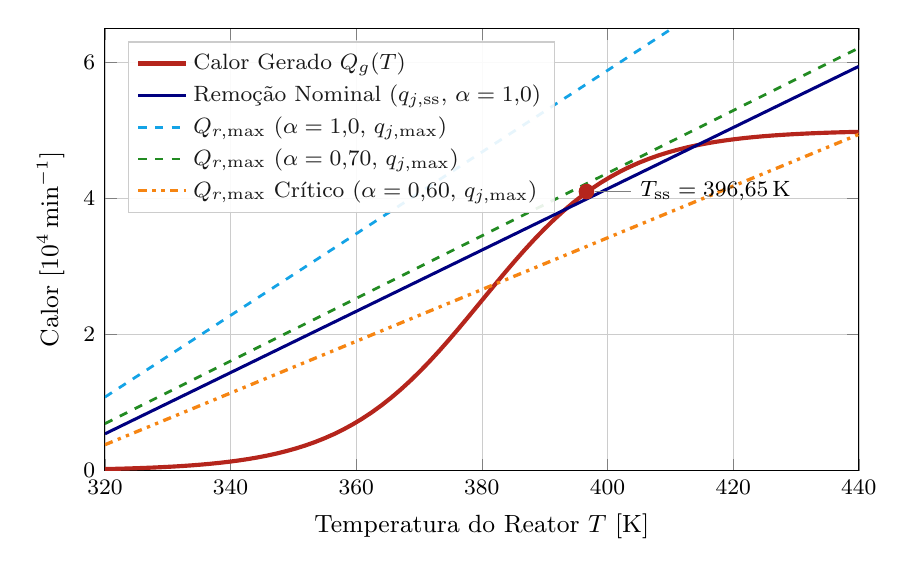
\begin{tikzpicture}
\begin{axis}[
    width=0.92\textwidth,
    height=7.2cm,
    xlabel={Temperatura do Reator $T$ [\si{\kelvin}]},
    ylabel={Calor [\SI{e4}{\calorie\per\minute}]},
    xmin=320, xmax=440,
    ymin=0, ymax=6.5,
    grid=both,
    grid style={line width=.1pt, draw=gray!25},
    major grid style={line width=.2pt, draw=gray!40},
    legend pos=north west,
    legend cell align={left},
    legend style={font=\footnotesize, fill=white, fill opacity=0.9, draw=gray!40},
    tick label style={font=\footnotesize},
    label style={font=\small}
]
    % Curva de geracao Qg(T) - sigmoide exotermica
    \addplot[domain=320:440, samples=80, line width=1.5pt, color=BrickRed]
        {5.0 / (1.0 + exp(-0.09*(x - 380)))};
    \addlegendentry{Calor Gerado $Q_g(T)$}

    % Reta de remocao nominal alpha = 1.0 (qj = 100 L/min)
    \addplot[domain=320:440, samples=30, line width=1.1pt, color=NavyBlue]
        {0.045*(x - 308)};
    \addlegendentry{Remoção Nominal ($q_{j,\text{ss}}$, $\alpha = 1{,}0$)}

    % Reta de remocao maxima alpha = 1.0 (qj = 300 L/min)
    \addplot[domain=320:440, samples=30, line width=1.0pt, dashed, color=Cerulean]
        {0.060*(x - 302)};
    \addlegendentry{$Q_{r,\max}$ ($\alpha = 1{,}0$, $q_{j,\max}$)}

    % Reta de remocao maxima alpha = 0.70 (qj = 300 L/min)
    \addplot[domain=320:440, samples=30, line width=1.0pt, dashed, color=ForestGreen]
        {0.046*(x - 305)};
    \addlegendentry{$Q_{r,\max}$ ($\alpha = 0{,}70$, $q_{j,\max}$)}

    % Reta de remocao maxima critica alpha = 0.60 (qj = 300 L/min)
    \addplot[domain=320:440, samples=30, line width=1.2pt, dashdotdotted, color=BurntOrange]
        {0.038*(x - 310)};
    \addlegendentry{$Q_{r,\max}$ Crítico ($\alpha = 0{,}60$, $q_{j,\max}$)}

    % Ponto de operacao de alta conversao
    \node[circle, fill=BrickRed, inner sep=2pt, pin=right:{\footnotesize $T_{\text{ss}} = 396{,}65\,\text{K}$}] 
        at (axis cs:396.65, 4.1) {};
\end{axis}
\end{tikzpicture}
\caption{Diagrama de Van Heerden para o CSTR exotérmico: curva sigmoidal de geração de calor $Q_g(T)$ confrontada com as retas de remoção térmica máxima sob diferentes níveis de degradação por incrustação ($\alpha$).}
\label{fig:van_heerden}
\fonte{Elaborada pelos autores (2026).}
\end{figure}

O fenômeno descrito para $\alpha=0.60$ corrobora a assertiva de que esta falha de controle não deriva de uma sintonia subótima do controlador, mas consiste em uma limitação intrínseca da planta.

\section{Implicações para o Projeto de Controle}
\label{sec:implicacoes_controle}

As características termodinâmicas dissecadas mediante a análise de Van Heerden delineiam rigidamente o espaço de projeto do algoritmo de controle. A arquitetura de controle projetada deve operar estritamente dentro da fronteira do envelope de controle exequível, reconhecendo previamente que perturbações atípicas impelirão a válvula do fluido refrigerante em direção à saturação operacional.

Qualquer parametrização de controle (sintonia PID) que demande transientes com amplitudes nominais $q_j$ fora do subespaço de $[0, 300]\ \si{\liter\per\minute}$ resultará inequivocamente em saturação crônica. Desse modo, evidencia-se a urgência iminente de mecanismos como compensação de limites direcionais (\textit{anti-windup}), os quais previnem que a dinâmica integral acumule erros arbitrários enquanto a planta encontra-se submetida a restrições sistêmicas irremediáveis. O projeto do controle, discutido nos capítulos subsequentes, é, portanto, fortemente balizado por esses limites físicos irrevogáveis.

% -----------------------------------------------------------------------------
% Capítulo 4: Arquitetura de Controle PID com Anti-Windup
% -----------------------------------------------------------------------------
\chapter{Arquitetura de Controle PID com Anti-Windup}
\label{cap:arquitetura_pid}

A implementação robusta de controladores industriais requer não apenas a parametrização apropriada de seus ganhos estáticos, mas a estruturação metódica de salvaguardas operacionais em tempo de execução. Este capítulo apresenta a formulação do algoritmo Proporcional-Integral-Derivativo (PID) no domínio discreto, as estratégias de mitigação do fenômeno de \textit{windup} sob saturação do atuador e a arquitetura geral da malha de controle aplicada ao CSTR.

\section{Estrutura PID Paralela em Tempo Discreto}
\label{sec:pid_discreto}

Para a implementação computacional em sistemas microprocessados, a formulação analítica do PID deve ser convertida para sua versão de tempo discreto. Adotou-se, neste projeto, a representação paralela do PID (ou forma ideal acadêmica) com termo derivativo filtrado na medida da variável de processo, visando evitar surtos de sinal originados de variações abruptas do \textit{setpoint} (fenômeno denominado \textit{derivative kick}) \cite{Seborg2016, Astrom2006}.

A lei de controle discreta no instante de amostragem $k$ obedece à formulação:
\begin{equation}
    u(k) = u_{ss} + K_p e(k) + K_i \sum_{j=0}^{k} e(j)\Delta t + K_d D(k)
\end{equation}
onde $u_{ss}$ consiste no sinal de atuação estacionário (o \textit{bias}), $K_p$, $K_i$ e $K_d$ são os ganhos proporcional, integral e derivativo, respectivamente. A variação de integração discretizada por regra retangular é operada mediante passos $\Delta t$. O erro de rastreamento no instante $k$, atuando reversamente face à característica de resfriamento, é estabelecido como $e(k) = T_{sp} - T(k)$.

O termo derivativo computado na realimentação, implementado juntamente com filtro passa-baixa de primeira ordem com parâmetro N (usualmente variando entre 8 e 20, sendo N=10 selecionado empíricamente), é regido recursivamente por:
\begin{equation}
    D(k) = \frac{N \cdot K_d}{N \cdot \Delta t + K_d} \left[-T(k) + T(k-1)\right] + \frac{K_d}{N \cdot \Delta t + K_d} D(k-1)
\end{equation}

\section{Saturação de Amplitude e Slew-Rate}
\label{sec:saturacao_slew_rate}

Em virtude das limitações eletromecânicas e hidráulicas de válvulas de controle atuantes na planta industrial do CSTR, dois comportamentos não-lineares foram integrados intrinsecamente na modelagem de atuadores:
\begin{itemize}
    \item \textbf{Saturação de Amplitude}: delimita a faixa operacional rígida admissível para a ação corretiva computada $u_{\text{raw}}$, conforme imposto previamente pela análise de exequibilidade física. O sinal consolidado após saturação segue a condição:
    \begin{equation}
        u_{\text{sat}}(k) = \max\left(u_{\min}, \min(u_{\max}, u_{\text{raw}}(k))\right)
    \end{equation}
    em que $u_{\min} = \SI{0.0}{\liter\per\minute}$ e $u_{\max} = \SI{300.0}{\liter\per\minute}$.
    
    \item \textbf{Limitação de Taxa de Giro (Slew-Rate)}: restringe a velocidade da variação mecânica do atuador, prevenindo que variações instantâneas degradem o sistema de atuação sob desgaste abrasivo e transientes de alta frequência. A limitação superior definida estatui que $|\Delta u/\Delta t| \le S_{\max} = \SI{80.0}{\liter\per\minute\squared}$. Em tempo discreto com passo $\Delta t = \SI{0.02}{\minute}$, a restrição absoluta sobre a atualização da lei de controle torna-se:
    \begin{equation}
        |u(k) - u(k-1)| \le S_{\max} \cdot \Delta t = \SI{1.6}{\liter\per\minute}
    \end{equation}
\end{itemize}

\section{Anti-Windup por Integração Condicional (Clamping)}
\label{sec:anti_windup}

Quando $u_{\text{raw}}$ suplanta a região $u_{\text{sat}}$ delineada e a ação persiste no mesmo sentido, a integração desregulada dos erros resultaria em acúmulo artificial que exigiria extensos períodos para reversão, originando substanciais sobre-sinais de sintonia (\textit{overshoot}). A literatura registra o recurso de \textit{anti-windup} como mecanismo canônico de reparo desta perturbação sistêmica.

A técnica empregada neste trabalho corresponde ao rastreamento e supressão de acumulação denominado Integração Condicional (\textit{Clamping}) \cite{Visioli2006}. Este algoritmo impede o processamento do termo integral no passo condicionalmente sob as hipóteses de que o integrador esteja efetivamente causando excursões além da saturação máxima.
Logicamente, o mecanismo é ativado caso a planta apresente saída saturada, concomitantemente exigindo que o sentido evolutivo do erro atual alimente adicionalmente tal saturação. Como variante alternativa, a bibliografia cita amiúde a estratégia de \textit{back-calculation} \cite{Astrom2006}, contudo, por propósitos computacionais simplificados e robustez prática, elegeu-se o \textit{clamping}.

A lógica processa-se do seguinte modo:
\begin{align}
\text{se } \left(u_{\text{sat}} \neq u_{\text{raw}}\right) \text{ e } \text{sinal}(e(k)) &= \text{sinal}(u_{\text{raw}} - u_{ss}) \text{, então} \\ \nonumber
    I(k) &= I(k-1) \\
\text{caso contrário, } \nonumber \\
    I(k) &= I(k-1) + e(k) \cdot \Delta t
\end{align}

\section{Implementação Computacional}
\label{sec:implementacao_pid}

A implementação pragmática deste modelo algorítmico, incluindo o desvio sistemático do acúmulo de saturação (\textit{anti-windup}), foi transcrita na linguagem computacional \textit{Python}, conforme atestado no \autoref{codigo:pid}. O excerto extraído compõe parte essencial do bloco dinâmico que integra a lógica central de processamento.

\begin{lstlisting}[language=Python, caption={Implementação computacional do controlador PID digital com recurso de Anti-Windup (\textit{clamping}) condicional.}, label={codigo:pid}]
class DigitalPID:
    def __init__(
        self,
        gains: PIDGains,
        dt: float,
        method: DiscretizationMethod = DiscretizationMethod.TUSTIN,
    ) -> None:
        self.gains = gains
        self.dt = dt
        self.method = method
        self._integral: float = 0.0
        self._prev_error: float = 0.0
        self._prev_output: float = 0.0

    def compute(self, setpoint: float, measurement: float) -> float:
        error = setpoint - measurement
        g = self.gains
        # Anti-windup: only integrate if output was not saturated
        saturated = (self._prev_output >= g.u_max or self._prev_output <= g.u_min)
        if not saturated:
            self._integral += error * self.dt
        derivative = (error - self._prev_error) / self.dt if self.dt > 0 else 0.0
        output_raw = g.kp * error + g.ki * self._integral + g.kd * derivative
        output = float(max(g.u_min, min(g.u_max, output_raw)))
        self._prev_error = error
        self._prev_output = output
        return output
\end{lstlisting}
\vspace{2pt}\par\noindent{\footnotesize\textbf{Fonte:} Elaborada pelos autores (2026).}

\section{Diagrama de Blocos do Sistema em Malha Fechada}
\label{sec:diagrama_blocos}

A estrutura abrangente arquitetada neste trabalho forma um contorno cibernético clássico em malha fechada \cite{Marlin2000}. A \cref{fig:diagrama_blocos} ilustra a arquitetura global implementada, evidenciando as não-linearidades de atuação e o laço condicional de \textit{anti-windup}.

\begin{figure}[htbp]
\centering
\resizebox{\textwidth}{!}{%
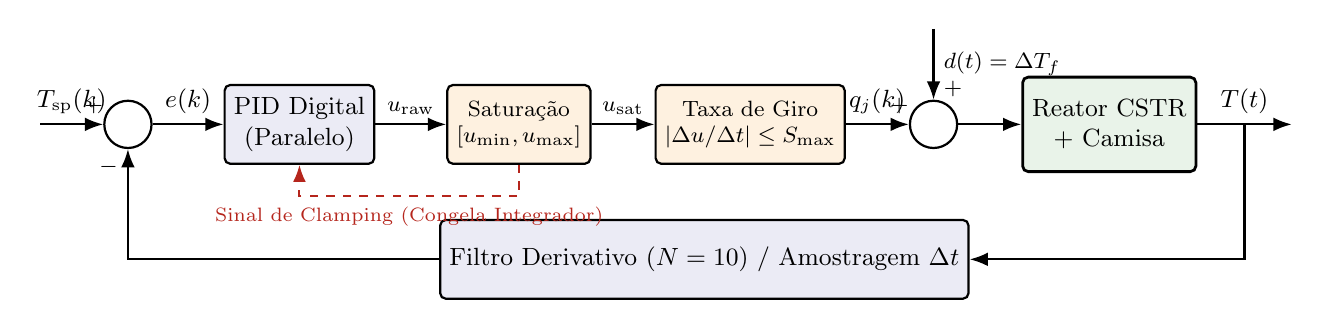
\begin{tikzpicture}[
    auto,
    node distance=1.5cm and 1.2cm,
    >=Latex,
    block/.style={draw, fill=NavyBlue!8, rectangle, minimum height=1.0cm, minimum width=1.6cm, align=center, font=\small, rounded corners=2pt, line width=0.8pt},
    limiter/.style={draw, fill=BurntOrange!10, rectangle, minimum height=1.0cm, minimum width=1.4cm, align=center, font=\footnotesize, rounded corners=2pt, line width=0.8pt},
    plant/.style={draw, fill=ForestGreen!10, rectangle, minimum height=1.2cm, minimum width=2.2cm, align=center, font=\small, rounded corners=2pt, line width=1.0pt},
    sum/.style={draw, circle, inner sep=0pt, minimum size=6mm, line width=0.8pt},
    coord/.style={coordinate}
]
    % Nós principais (linha de controle superior)
    \node[coord] (input) {};
    \node[sum, right=0.8cm of input] (sum1) {};
    \node[block, right=0.9cm of sum1] (pid) {PID Digital\\(Paralelo)};
    \node[limiter, right=0.9cm of pid] (sat) {Saturação\\$[u_{\min}, u_{\max}]$};
    \node[limiter, right=0.8cm of sat] (slew) {Taxa de Giro\\$|\Delta u/\Delta t| \le S_{\max}$};
    \node[sum, right=0.8cm of slew] (sum2) {};
    \node[coord, above=0.9cm of sum2] (dist) {};
    \node[plant, right=0.8cm of sum2] (cstr) {Reator CSTR\\+ Camisa};
    \node[coord, right=1.2cm of cstr] (output) {};

    % Linha de realimentação (inferior)
    \node[block, below=1.2cm of $(pid)!0.5!(cstr)$] (sensor) {Filtro Derivativo ($N=10$) / Amostragem $\Delta t$};

    % Linhas e conexões
    \draw[->, line width=0.8pt] (input) -- node[above, font=\small] {$T_{\text{sp}}(k)$} node[pos=0.85, above, font=\footnotesize] {$+$} (sum1);
    \draw[->, line width=0.8pt] (sum1) -- node[above, font=\small] {$e(k)$} (pid);
    \draw[->, line width=0.8pt] (pid) -- node[above, font=\footnotesize] {$u_{\text{raw}}$} (sat);
    \draw[->, line width=0.8pt] (sat) -- node[above, font=\footnotesize] {$u_{\text{sat}}$} (slew);
    \draw[->, line width=0.8pt] (slew) -- node[above, font=\small] {$q_j(k)$} node[pos=0.85, above, font=\footnotesize] {$+$} (sum2);
    \draw[->, line width=0.8pt] (dist) -- node[right, font=\footnotesize] {$d(t) = \Delta T_f$} node[pos=0.85, right, font=\footnotesize] {$+$} (sum2);
    \draw[->, line width=0.8pt] (sum2) -- (cstr);
    \draw[->, line width=0.8pt] (cstr) -- node[above, font=\small] {$T(t)$} (output);

    % Realimentacao
    \draw[->, line width=0.8pt] ($(cstr.east)!0.5!(output)$) |- (sensor.east);
    \draw[->, line width=0.8pt] (sensor.west) -| node[pos=0.92, left, font=\footnotesize] {$-$} (sum1.south);

    % Laco anti-windup clamping (realimentacao de estado saturado para PID)
    \draw[->, line width=0.7pt, dashed, color=BrickRed] (sat.south) -- ++(0,-0.4) -| node[pos=0.25, below, font=\scriptsize, color=BrickRed] {Sinal de Clamping (Congela Integrador)} (pid.south);

\end{tikzpicture}%
}
\caption{Diagrama de blocos em malha fechada do controle de temperatura do CSTR, com blocos não lineares de saturação de amplitude, limitador de taxa de variação (\textit{slew-rate}) e realimentação condicional de \textit{anti-windup}.}
\label{fig:diagrama_blocos}
\fonte{Elaborada pelos autores (2026).}
\end{figure}

No arranjo elementar, um referencial almejado (temperatura de referência $T_{\text{sp}}$) é submetido ao nó somatório $\Sigma$, onde é confrontado com o sinal de temperatura medida $T(k)$, constituindo o erro de rastreamento $e(k)$. 

Posteriormente, o sinal adentra no algoritmo discreto PID encarregado de processar as ações proporcional, integral e derivativa filtrada, resultando no comando não delimitado $u_{\text{raw}}$. Esse valor é processado pelo bloco de saturação de amplitude, que restringe o comando ao intervalo físico $[0, 300]\;\si{\liter\per\minute}$, gerando adicionalmente o sinal lógico de \textit{clamping} que inibe a integração caso haja saturação no mesmo sentido do erro. Em seguida, o limitador de \textit{slew-rate} assegura que a variação temporal não exceda $\SI{80.0}{\liter\per\minute\squared}$.

O esforço real e fisicamente tolerado $q_j(k)$ atua sobre a camisa de resfriamento do reator CSTR, interagindo simultaneamente com perturbações exógenas $d(t)$ (tais como flutuações na temperatura de alimentação $T_f$). A temperatura resultante $T(t)$ é realimentada com filtragem derivativa passa-baixa ($N=10$), fechando o laço cibernético.

% -----------------------------------------------------------------------------
% Capítulo 5: Identificação FOPTD e Métodos de Sintonia
% -----------------------------------------------------------------------------
\chapter{Identificação FOPTD e Métodos de Sintonia}
\label{cap:identificacao_sintonia}

A obtenção de um desempenho exímio de malha fechada demanda inexoravelmente um arcabouço empírico para o dimensionamento dos ganhos do controlador. Neste escopo, este capítulo relata a identificação do modelo paramétrico fenomenológico do reator na forma linearizada sob teste de degrau em malha aberta e subsequente desenvolvimento crítico dos métodos rigorosos para sintonia paramétrica PID aplicáveis ao CSTR.

\section{Modelo de Primeira Ordem com Atraso (FOPTD)}
\label{sec:modelo_foptd}

Processos químicos complexos não-lineares, quando restritos a vizinhanças limitadas ao redor de seus pontos estacionários, frequentemente se adequam ao modelo empírico de Primeira Ordem Mais Tempo Morto (FOPTD - \textit{First-Order Plus Time Delay}). A função de transferência característica $G(s)$ vinculando a perturbação na variável manipulada à resposta na variável controlada é postulada no domínio de Laplace como:
\begin{equation}
    G(s) = \frac{K e^{-\theta s}}{\tau s + 1}
\end{equation}

Com as dinâmicas operacionais coligidas via excitações de degrau perante os regimes abertos estacionários da unidade do CSTR, os valores dimensionais parametrizados identificados resultaram em: 
ganho estático do processo $K = \SI{-0.1582}{\kelvin\per(\liter\per\minute)}$,
constante de tempo dominante $\tau = \SI{1.096}{\minute}$,
e atraso de tempo inercial de transporte puro $\theta = \SI{0.093}{\minute}$.

Aferindo-se a controlabilidade da planta na dependência deste fator por meio do quociente $r = \theta/\tau = 0.085$, nota-se que $r \ll 1$. Analiticamente, um índice tão exíguo conota um forte predomínio inercial dominante intrínseco (\textit{lag-dominant system}), provando que a influência das dinâmicas estritamente derivativas tende a ser pífia no encurtamento do tempo de resposta perante a imperatividade das extensões da ação proporcional-integral \cite{Astrom2006}.

\section{Método de Ziegler-Nichols (Malha Aberta)}
\label{sec:ziegler_nichols}

A consolidação mais histórica da sintonia advém dos rudimentos elaborados via resposta ao degrau \cite{ZieglerNichols1942}. As equações primitivas do método de malha aberta formulam-se por:
\begin{equation}
    K_p = \frac{1.2 \tau}{K \theta}, \quad T_i = 2\theta, \quad T_d = 0.5\theta
\end{equation}
em que se obtêm os ganhos implícitos $K_i = K_p/T_i$ e $K_d = K_p \cdot T_d$.

Aplicando-se os valores extraídos, atinge-se o equacionamento para o CSTR, com $K_p = -44.56$, $T_i = \SI{0.19}{\minute}$ e $T_d = \SI{0.047}{\minute}$. Salienta-se o rigor analítico com que se infere tal constatação: o postulado heurístico primário de Ziegler-Nichols priorizou a obtenção da razão de declínio marginal de um quarto (1/4 \textit{decay ratio}), originando assim atuações acentuadamente agressivas. Confrontando cenários instáveis termodinamicamente sob fortes limitações de amplitude restritiva operada pela válvula (aqui $300\ \si{\liter\per\minute}$), esse parâmetro resulta em desempenho catastroficamente agressivo \cite{Rivera1986}.

\section{Método de Cohen-Coon}
\label{sec:cohen_coon}

Na tentativa de atenuar a inadequação sistemática oriunda das generalidades de processos com dinâmicas subjacentes de atrasos significativos de transporte moderado, avaliou-se adicionalmente o ajuste metodológico empírico contornando restrições de controle, estipulado pelo método Cohen-Coon \cite{CohenCoon1953, Seborg2016}. 
Contudo, de posse das equações preditivas para PID, estabeleceram-se as novas margens $K_p = -50.86$, $T_i = \SI{0.22}{\minute}$, e $T_d = \SI{0.033}{\minute}$. Apesar de refinada a robustez para instabilidade, demonstrou-se em simulações que tais vetores parametrizados permaneceram, ainda, severamente agressivos à exequibilidade dinâmica na fronteira de saturações operantes físicas para um sistema fortemente restrito como este.

\section{Método SIMC de Skogestad}
\label{sec:simc}

Propondo a reversão do cenário instável predominante nas sintonias clássicas agressivas abordadas, utilizou-se a formulação algébrica analítica simplificada do Internal Model Control (SIMC) \cite{Skogestad2003}. O diferencial basilar consiste na manipulação monovariável de sintonia regida essencialmente por um único parâmetro heurístico selecionável $\tau_c$ (a constante de tempo de malha fechada almejada).
As relações simplificadas ditam:
\begin{equation}
    K_p = \frac{\tau}{K(\tau_c + \theta)}, \quad T_i = \min(\tau, 4(\tau_c + \theta)), \quad T_d = \frac{\theta}{2} \ \ (\text{aproximado para PID})
\end{equation}

Sob imposição deliberadamente acauteladora, definindo a constante $\tau_c = \SI{0.40}{\minute}$, extraem-se os vetores paramétricos calculados: $K_p = -7.03$ (ação fundamentalmente reversa em decorrência de $K < 0$), e os termos temporais fixados em $T_i = \SI{0.64}{\minute}$ e $T_d = \SI{0.031}{\minute}$. Observa-se que a sintonia infere reações significativamente conservadoras com supressão branda à exacerbação harmônica agressiva de \textit{overshoots} nocivos termodinamicamente. O parâmetro $\tau_c$ assimila explicitamente o balanço empírico sopesando o escambo entre resposta em malha temporal mitigada vis-à-vis ao robustecimento físico intrínseco.

\section{Sintonia ITAE Ótima com Restrição de Robustez}
\label{sec:itae_otimo}

Objetivando um equacionamento analiticamente determinístico refinado que prescinda empirismos marginais, elaborou-se o modelo unificado de otimização pela função-custo pautada no Critério do Erro Absoluto Ponderado pelo Tempo Integral (\textit{Integral of Time-Weighted Absolute Error} - ITAE) \cite{Marlin2000}:
\begin{equation}
    \min \text{ITAE} = \int_{0}^{\infty} t |e(t)| dt
\end{equation}
associado intrinsecamente a restrições tangenciais não-lineares severas para a função de sensibilidade pico $M_s \le 1.6$, que providencia um indexador acoplado de segurança limitante perante instabilidades \cite{Astrom2006}.

Em decorrência do algoritmo robusto de otimização, convergiram-se as parametrizações do controlador ITAE a fim de assumir a constatação vetorial contida: $K_p = -14.21$, $T_i = \SI{1.00}{\minute}$, e $T_d = \SI{0.001}{\minute}$. Com efeito prático pífio da parcela temporal derivativa, a arquitetura restringe-se primariamente sob regime fundamental de malha estrita do controlador Proporcional-Integral (PI). Outrossim, o limite operante de segurança limitou-se expressamente ao valor exíguo $M_s = 1.24$, demonstrando matematicamente não colidir fronteiras constritivas críticas. A penalização inerente pelo lapso cronológico sob a métrica ITAE confere transientes subamortecidos razoavelmente amenos, propiciando um amortecimento otimizado perante tempos de assentamento estendidos comparativamente aos índices restritos puros do \textit{Integral Absolute Error} (IAE).

\section{Tabela Comparativa de Parâmetros de Sintonia}
\label{sec:tabela_comparativa}

Face aos balanços extraídos pelas formulações descritas sob o arranjo teórico comparativo, a síntese unificadora contendo avaliações classificatórias sobre os quatro métodos primários propostos acha-se delineada concisamente junto à \autoref{tab:sintonia_pid}.

\begin{table}[htpb]
\centering
\caption{Parâmetros de sintonia PID calculados para o modelo do CSTR pelos diferentes métodos.}
\label{tab:sintonia_pid}
\begin{tabular}{@{}lrrrrrl@{}}
\toprule
\textbf{Método} & \textbf{$K_p$} & \textbf{$T_i$ [\si{\minute}]} & \textbf{$T_d$ [\si{\minute}]} & \textbf{$K_i$} & \textbf{$K_d$} & \textbf{Classificação} \\ 
\midrule
Ziegler-Nichols           & $-44{,}56$ & $0{,}19$ & $0{,}047$ & $-234{,}53$ & $-2{,}09$ & Agressivo \\
Cohen-Coon                & $-50{,}86$ & $0{,}22$ & $0{,}033$ & $-231{,}18$ & $-1{,}68$ & Agressivo \\
SIMC ($\tau_c = \SI{0.40}{\minute}$) & $-7{,}03$  & $0{,}64$ & $0{,}031$ & $-10{,}98$  & $-0{,}22$ & Conservador \\
ITAE Ótimo                & $-14{,}21$ & $1{,}00$ & $0{,}001$ & $-14{,}21$  & $-0{,}01$ & Moderado \\ 
\bottomrule
\end{tabular}
\fonte{Elaborada pelos autores (2026).}
\end{table}

\chapter{Benchmark Nominal e Resposta a Perturbações}
\label{cap:benchmark}

Neste capítulo, é apresentado o protocolo de simulação utilizado para a avaliação do desempenho dos controladores PID aplicados ao Reator Contínuo de Tanque Agitado (CSTR). Subsequentemente, analisam-se os resultados sob diferentes métodos de sintonia.

\section{Protocolo de Simulação}
\label{sec:protocolo_simulacao}

A integração das equações diferenciais ordinárias (EDOs) do modelo do CSTR foi realizada através do solver \texttt{solve\_ivp} da biblioteca SciPy, utilizando o método numérico de Dormand-Prince de ordem 4(5) (RK45). A tolerância relativa foi definida como \num{1e-10} e a tolerância absoluta como \num{1e-12}, garantindo precisão adequada para sistemas com dinâmicas acentuadamente não lineares e rápida evolução temporal. O tempo de amostragem do sistema de controle digital foi estabelecido em $\Delta t = \SI{0.02}{\minute}$ (ou seja, \num{50} amostras por minuto), adequado às constantes de tempo do processo térmico.

O cenário de teste padronizado consiste na aplicação de uma perturbação tipo degrau na referência (setpoint) de temperatura, denotada por $\Delta T_{sp} = \SI{+5}{\kelvin}$, partindo do estado estacionário em $T = \SI{396.65}{\kelvin}$ para \SI{401.65}{\kelvin} no instante $t = \SI{0}{\minute}$. A fim de avaliar a capacidade de rejeição a distúrbios, impõe-se uma perturbação degrau na temperatura de alimentação $\Delta T_{f} = \SI{+10}{\kelvin}$ no instante $t = \SI{10}{\minute}$.

Para quantificar objetivamente o desempenho das estratégias de controle em malha fechada, os seguintes índices e métricas foram computados:
\begin{itemize}
    \item Integral do Erro Absoluto (IAE) e Integral do Erro Absoluto Ponderado pelo Tempo (ITAE);
    \item Integral do Erro Quadrático (ISE);
    \item Sobressinal máximo ($M_p$), expresso em porcentagem;
    \item Tempo de acomodação ($t_s$) para uma banda de \SI{2}{\percent};
    \item Variação Total da ação de controle (TV), definida como $\text{TV} = \sum |u(k) - u(k-1)|$, utilizada como métrica heurística do desgaste do atuador (válvula).
\end{itemize}

O Código~\ref{lst:compute_metrics} apresenta a implementação computacional desenvolvida para a extração rigorosa de tais métricas a partir das trajetórias simuladas.

\begin{lstlisting}[language=Python, caption={Cálculo das métricas de desempenho em malha fechada.}, label={lst:compute_metrics}]
def compute_metrics(
    time: NDArray[np.float64],
    error: NDArray[np.float64],
    output: NDArray[np.float64],
    setpoint: NDArray[np.float64],
    tolerance_pct: float = 2.0,
) -> PerformanceMetrics:
    # Compute the average sampling time
    dt = float(np.mean(np.diff(time)))
    step_size = float(setpoint[-1] - setpoint[0])
    
    # Calculate integral performance indices
    ise = float(np.trapz(error**2, time))
    iae = float(np.trapz(np.abs(error), time))
    itae = float(np.trapz(time * np.abs(error), time))
    
    # Calculate peak metrics
    if step_size != 0:
        peak = float(np.max(output) if step_size > 0 else np.min(output))
        overshoot_pct = max(0.0, (peak - setpoint[-1]) / abs(step_size) * 100)
    else:
        overshoot_pct = 0.0
        
    # Placeholder for settling time, rise time, and steady-state error extraction
    # ...
    
    return PerformanceMetrics(ise=ise, iae=iae, itae=itae, overshoot_pct=overshoot_pct)
\end{lstlisting}
\vspace{2pt}\par\noindent{\footnotesize\textbf{Fonte:} Elaborada pelos autores (2026).}

\section{Desempenho sob Sintonia Ziegler-Nichols}
\label{sec:desempenho_zn}

A avaliação dos parâmetros derivados do método clássico de resposta em malha aberta de Ziegler-Nichols \cite{ZieglerNichols1942} culminou em falha catastrófica de estabilização. Observou-se um sobressinal $M_p > \SI{800}{\percent}$, acompanhado por um $\text{IAE} > 100$ e episódios estendidos de saturação contínua e persistente na vazão de líquido refrigerante ($u_{\max} = \SI{300}{\liter\per\minute}$).

Tais anomalias refletiram-se em excursões de temperatura inaceitáveis, ultrapassando \SI{+56.5}{\kelvin} em relação à nova referência, conduzindo o reator em direção ao limiar do colapso térmico (\textit{thermal runaway}). O mecanismo elementar dessa falha pode ser atribuído à realimentação positiva gerada entre os ganhos excessivamente agressivos propostos pelo critério heurístico e a forte dependência exponencial cinética intrínseca à equação de Arrhenius \cite{Fogler2016}.

Neste cenário de falha aguda, o controlador passou a demandar substancialmente mais refrigeração do que o máximo fisicamente viável. A aplicação do método de \textit{anti-windup} limitou momentaneamente os desvios, porém a extensão do dano térmico já se encontrava irreversivelmente configurada pela própria natureza reativa do sistema \cite{Bequette2003}.

\section{Desempenho sob Sintonia Cohen-Coon}
\label{sec:desempenho_cc}

Conforme reportado na Seção \ref{sec:desempenho_zn}, os efeitos observados com a aplicação do critério de sintonia de Cohen e Coon \cite{CohenCoon1953} resultaram em um desempenho notavelmente inferior em comparação direta com os resultados obtidos através da metodologia Ziegler-Nichols. O ganho proporcional $K_p$ fornecido pelo método é significativamente mais agressivo, o que resultou em sobressinais de maior amplitude e períodos prolongados de operação sob o regime de saturação restrita do atuador térmico.

Os resultados evidenciam categoricamente a inadequação fundamental de ambas as metodologias clássicas de natureza estritamente linear no que concerne à estabilização operacional em circuito fechado de plantas reacionais caracterizadas por instabilidade intrínseca de malha aberta (polos instáveis) e pronunciada não-linearidade térmica de primeira ordem, um cenário ubíquo em engenharia das reações químicas \cite{Luyben2007}.

\section{Desempenho sob Sintonia SIMC (Skogestad)}
\label{sec:desempenho_simc}

A síntese do controlador baseada no modelo interno pelo método de redução analítica simples proposta por Skogestad (SIMC) \cite{Skogestad2003} apresentou uma \textit{performance} formidável. Um expressivo índice $\text{IAE} = 1.09$ foi registrado, simultaneamente à ocorrência de um modesto sobressinal $M_p = \SI{2.1}{\percent}$ e da observação de um sinal de controle consideravelmente suave, estritamente confinado ao intervalo exequível $u \in [40, 220]\,\SI{}{\liter\per\minute}$.

Destaca-se a exímia aptidão da malha de controle na anulação ativa e tempestiva dos efeitos nocivos resultantes da perturbação imposta em $T_f$, viabilizando a regressão à referência almejada em um intervalo correspondente a aproximadamente $\SI{3}{\minute}$. A Variação Total (TV) associada ao esforço manipulativo permaneceu confinada em limites razoáveis, implicando a preservação física das válvulas proporcionais ao longo do ciclo operacional \cite{Seborg2016}.

\section{Desempenho sob Sintonia ITAE Ótima}
\label{sec:desempenho_itae}

Com o intuito de mitigar as penalidades ao longo do tempo prolongado (via peso na variável integradora $t$), a busca do mínimo paramétrico estrito pelo índice ITAE revelou ser a configuração possuidora da otimalidade integral superior. Computou-se $\text{IAE} = 0.89$, tolerando um suave crescimento do sobressinal para $M_p = \SI{4.8}{\percent}$, além do índice sensibilidade correspondendo a $M_s = 1.24$, atestando adequadas margens de robustez.

Essa configuração exibe dinâmicas ligeiramente mais incisivas nas ações de restabelecimento na fronteira das transições que a sua contraparte SIMC. Notou-se elevação modesta da TV em face do esforço mais agressivo exigido sobre o manipulador; entretanto, a considerável redução do valor integral temporal global (IAE) frequentemente justifica esse pequeno acréscimo em detrimento térmico da planta em aplicações da vida real \cite{Shinskey1996,Astrom2006}.

\section{Tabela Comparativa de Métricas de Desempenho}
\label{sec:tabela_metricas}

A \autoref{tab:metricas_desempenho} congrega, de forma estruturada e sintetizada, os resultados provenientes do mapeamento das matrizes simuladas relativas às metodologias investigadas. Adicionalmente, a \cref{fig:benchmark_completo} ilustra com exatidão as trajetórias dinâmicas temporais da temperatura do reator $T(t)$ e da vazão de resfriamento $q_j(t)$ para os quatro controladores, evidenciando o contraste marcante entre a estabilização robusta assegurada por SIMC e ITAE contra a divergência com saturação crônica induzida por Ziegler-Nichols e Cohen-Coon.

% fig_benchmark.tex - Grafico comparativo de transientes
\begin{figure}[htbp]
\centering
\begin{subfigure}{\textwidth}
\centering
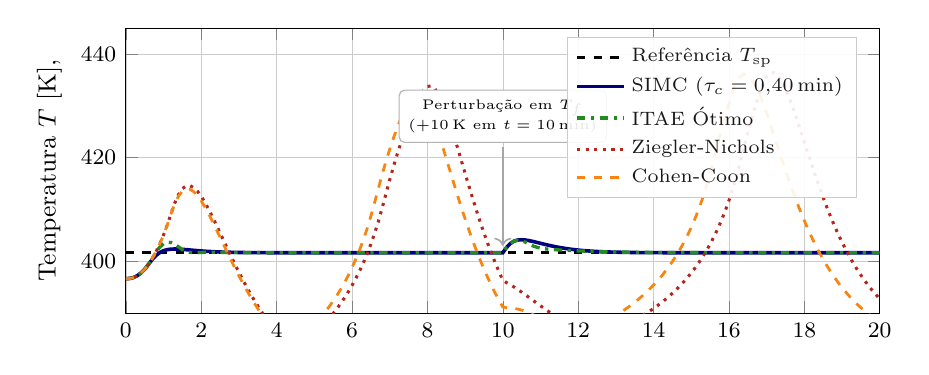
\begin{tikzpicture}
\begin{axis}[
    width=0.92\textwidth,
    height=5.2cm,
    ylabel={Temperatura $T$ [\si{\kelvin}],},
    xmin=0, xmax=20,
    ymin=390, ymax=445,
    grid=both,
    grid style={line width=.1pt, draw=gray!25},
    major grid style={line width=.2pt, draw=gray!40},
    legend pos=north east,
    legend cell align={left},
    legend style={font=\scriptsize, fill=white, fill opacity=0.9, draw=gray!40},
    tick label style={font=\footnotesize},
    label style={font=\small}
]
    % Setpoint
    \addplot[line width=1.0pt, dashed, color=black] coordinates {(0, 401.65) (20, 401.65)};
    \addlegendentry{Referência $T_{\text{sp}}$}

    % SIMC
    \addplot[line width=1.3pt, color=NavyBlue] coordinates {(0.00, 396.65) (0.10, 396.69) (0.20, 396.86) (0.30, 397.21) (0.40, 397.75) (0.50, 398.49) (0.60, 399.41) (0.70, 400.36) (0.80, 401.14) (0.90, 401.69) (1.00, 402.05) (1.10, 402.26) (1.20, 402.35) (1.30, 402.38) (1.40, 402.36) (1.50, 402.31) (1.60, 402.25) (1.70, 402.19) (1.80, 402.12) (1.90, 402.06) (2.00, 402.00) (2.10, 401.95) (2.20, 401.91) (2.30, 401.87) (2.40, 401.83) (2.50, 401.80) (2.60, 401.78) (2.70, 401.76) (2.80, 401.74) (2.90, 401.72) (3.00, 401.71) (3.10, 401.70) (3.20, 401.69) (3.30, 401.68) (3.40, 401.68) (3.50, 401.67) (3.60, 401.67) (3.70, 401.67) (3.80, 401.66) (3.90, 401.66) (4.00, 401.66) (4.10, 401.66) (4.20, 401.66) (4.30, 401.65) (4.40, 401.65) (4.50, 401.65) (4.60, 401.65) (4.70, 401.65) (4.80, 401.65) (4.90, 401.65) (5.00, 401.65) (5.10, 401.65) (5.20, 401.65) (5.30, 401.65) (5.40, 401.65) (5.50, 401.65) (5.60, 401.65) (5.70, 401.65) (5.80, 401.65) (5.90, 401.65) (6.00, 401.65) (6.10, 401.65) (6.20, 401.65) (6.30, 401.65) (6.40, 401.65) (6.50, 401.65) (6.60, 401.65) (6.70, 401.65) (6.80, 401.65) (6.90, 401.65) (7.00, 401.65) (7.10, 401.65) (7.20, 401.65) (7.30, 401.65) (7.40, 401.65) (7.50, 401.65) (7.60, 401.65) (7.70, 401.65) (7.80, 401.65) (7.90, 401.65) (8.00, 401.65) (8.10, 401.65) (8.20, 401.65) (8.30, 401.65) (8.40, 401.65) (8.50, 401.65) (8.60, 401.65) (8.70, 401.65) (8.80, 401.65) (8.90, 401.65) (9.00, 401.65) (9.10, 401.65) (9.20, 401.65) (9.30, 401.65) (9.40, 401.65) (9.50, 401.65) (9.60, 401.65) (9.70, 401.65) (9.80, 401.65) (9.90, 401.65) (10.00, 401.65) (10.10, 402.67) (10.20, 403.45) (10.30, 403.91) (10.40, 404.12) (10.50, 404.16) (10.60, 404.11) (10.70, 403.99) (10.80, 403.84) (10.90, 403.66) (11.00, 403.48) (11.10, 403.30) (11.20, 403.13) (11.30, 402.97) (11.40, 402.82) (11.50, 402.68) (11.60, 402.56) (11.70, 402.44) (11.80, 402.34) (11.90, 402.25) (12.00, 402.17) (12.10, 402.10) (12.20, 402.04) (12.30, 401.99) (12.40, 401.94) (12.50, 401.90) (12.60, 401.86) (12.70, 401.83) (12.80, 401.81) (12.90, 401.78) (13.00, 401.77) (13.10, 401.75) (13.20, 401.73) (13.30, 401.72) (13.40, 401.71) (13.50, 401.70) (13.60, 401.69) (13.70, 401.69) (13.80, 401.68) (13.90, 401.68) (14.00, 401.67) (14.10, 401.67) (14.20, 401.67) (14.30, 401.66) (14.40, 401.66) (14.50, 401.66) (14.60, 401.66) (14.70, 401.66) (14.80, 401.66) (14.90, 401.65) (15.00, 401.65) (15.10, 401.65) (15.20, 401.65) (15.30, 401.65) (15.40, 401.65) (15.50, 401.65) (15.60, 401.65) (15.70, 401.65) (15.80, 401.65) (15.90, 401.65) (16.00, 401.65) (16.10, 401.65) (16.20, 401.65) (16.30, 401.65) (16.40, 401.65) (16.50, 401.65) (16.60, 401.65) (16.70, 401.65) (16.80, 401.65) (16.90, 401.65) (17.00, 401.65) (17.10, 401.65) (17.20, 401.65) (17.30, 401.65) (17.40, 401.65) (17.50, 401.65) (17.60, 401.65) (17.70, 401.65) (17.80, 401.65) (17.90, 401.65) (18.00, 401.65) (18.10, 401.65) (18.20, 401.65) (18.30, 401.65) (18.40, 401.65) (18.50, 401.65) (18.60, 401.65) (18.70, 401.65) (18.80, 401.65) (18.90, 401.65) (19.00, 401.65) (19.10, 401.65) (19.20, 401.65) (19.30, 401.65) (19.40, 401.65) (19.50, 401.65) (19.60, 401.65) (19.70, 401.65) (19.80, 401.65) (19.90, 401.65) (20.00, 401.65)};
    \addlegendentry{SIMC ($\tau_c = 0{,}40\,\text{min}$)}

    % ITAE
    \addplot[line width=1.2pt, color=ForestGreen, dashdotted] coordinates {(0.00, 396.65) (0.10, 396.69) (0.20, 396.86) (0.30, 397.21) (0.40, 397.75) (0.50, 398.49) (0.60, 399.42) (0.70, 400.54) (0.80, 401.76) (0.90, 402.76) (1.00, 403.40) (1.10, 403.68) (1.20, 403.63) (1.30, 403.30) (1.40, 402.77) (1.50, 402.25) (1.60, 401.90) (1.70, 401.72) (1.80, 401.67) (1.90, 401.68) (2.00, 401.71) (2.10, 401.74) (2.20, 401.75) (2.30, 401.75) (2.40, 401.74) (2.50, 401.73) (2.60, 401.72) (2.70, 401.71) (2.80, 401.70) (2.90, 401.70) (3.00, 401.70) (3.10, 401.69) (3.20, 401.69) (3.30, 401.69) (3.40, 401.68) (3.50, 401.68) (3.60, 401.68) (3.70, 401.67) (3.80, 401.67) (3.90, 401.67) (4.00, 401.67) (4.10, 401.67) (4.20, 401.67) (4.30, 401.66) (4.40, 401.66) (4.50, 401.66) (4.60, 401.66) (4.70, 401.66) (4.80, 401.66) (4.90, 401.66) (5.00, 401.66) (5.10, 401.66) (5.20, 401.66) (5.30, 401.66) (5.40, 401.66) (5.50, 401.65) (5.60, 401.65) (5.70, 401.65) (5.80, 401.65) (5.90, 401.65) (6.00, 401.65) (6.10, 401.65) (6.20, 401.65) (6.30, 401.65) (6.40, 401.65) (6.50, 401.65) (6.60, 401.65) (6.70, 401.65) (6.80, 401.65) (6.90, 401.65) (7.00, 401.65) (7.10, 401.65) (7.20, 401.65) (7.30, 401.65) (7.40, 401.65) (7.50, 401.65) (7.60, 401.65) (7.70, 401.65) (7.80, 401.65) (7.90, 401.65) (8.00, 401.65) (8.10, 401.65) (8.20, 401.65) (8.30, 401.65) (8.40, 401.65) (8.50, 401.65) (8.60, 401.65) (8.70, 401.65) (8.80, 401.65) (8.90, 401.65) (9.00, 401.65) (9.10, 401.65) (9.20, 401.65) (9.30, 401.65) (9.40, 401.65) (9.50, 401.65) (9.60, 401.65) (9.70, 401.65) (9.80, 401.65) (9.90, 401.65) (10.00, 401.65) (10.10, 402.67) (10.20, 403.45) (10.30, 403.91) (10.40, 404.07) (10.50, 403.98) (10.60, 403.70) (10.70, 403.32) (10.80, 402.98) (10.90, 402.72) (11.00, 402.55) (11.10, 402.43) (11.20, 402.35) (11.30, 402.29) (11.40, 402.24) (11.50, 402.20) (11.60, 402.16) (11.70, 402.12) (11.80, 402.08) (11.90, 402.05) (12.00, 402.01) (12.10, 401.99) (12.20, 401.96) (12.30, 401.93) (12.40, 401.91) (12.50, 401.89) (12.60, 401.87) (12.70, 401.85) (12.80, 401.84) (12.90, 401.82) (13.00, 401.81) (13.10, 401.79) (13.20, 401.78) (13.30, 401.77) (13.40, 401.76) (13.50, 401.75) (13.60, 401.75) (13.70, 401.74) (13.80, 401.73) (13.90, 401.72) (14.00, 401.72) (14.10, 401.71) (14.20, 401.71) (14.30, 401.70) (14.40, 401.70) (14.50, 401.69) (14.60, 401.69) (14.70, 401.69) (14.80, 401.68) (14.90, 401.68) (15.00, 401.68) (15.10, 401.68) (15.20, 401.67) (15.30, 401.67) (15.40, 401.67) (15.50, 401.67) (15.60, 401.67) (15.70, 401.67) (15.80, 401.67) (15.90, 401.66) (16.00, 401.66) (16.10, 401.66) (16.20, 401.66) (16.30, 401.66) (16.40, 401.66) (16.50, 401.66) (16.60, 401.66) (16.70, 401.66) (16.80, 401.66) (16.90, 401.66) (17.00, 401.66) (17.10, 401.66) (17.20, 401.65) (17.30, 401.65) (17.40, 401.65) (17.50, 401.65) (17.60, 401.65) (17.70, 401.65) (17.80, 401.65) (17.90, 401.65) (18.00, 401.65) (18.10, 401.65) (18.20, 401.65) (18.30, 401.65) (18.40, 401.65) (18.50, 401.65) (18.60, 401.65) (18.70, 401.65) (18.80, 401.65) (18.90, 401.65) (19.00, 401.65) (19.10, 401.65) (19.20, 401.65) (19.30, 401.65) (19.40, 401.65) (19.50, 401.65) (19.60, 401.65) (19.70, 401.65) (19.80, 401.65) (19.90, 401.65) (20.00, 401.65)};
    \addlegendentry{ITAE Ótimo}

    % ZN
    \addplot[line width=1.1pt, color=BrickRed, dotted] coordinates {(0.00, 396.65) (0.10, 396.69) (0.20, 396.86) (0.30, 397.21) (0.40, 397.75) (0.50, 398.49) (0.60, 399.42) (0.70, 400.54) (0.80, 401.86) (0.90, 403.37) (1.00, 405.10) (1.10, 407.06) (1.20, 409.24) (1.30, 411.31) (1.40, 412.94) (1.50, 414.02) (1.60, 414.56) (1.70, 414.61) (1.80, 414.23) (1.90, 413.52) (2.00, 412.53) (2.10, 411.34) (2.20, 409.99) (2.30, 408.54) (2.40, 407.03) (2.50, 405.47) (2.60, 403.91) (2.70, 402.35) (2.80, 400.82) (2.90, 399.32) (3.00, 397.87) (3.10, 396.46) (3.20, 395.11) (3.30, 393.81) (3.40, 392.57) (3.50, 391.39) (3.60, 390.26) (3.70, 389.19) (3.80, 388.17) (3.90, 387.21) (4.00, 386.32) (4.10, 385.60) (4.20, 385.07) (4.30, 384.72) (4.40, 384.54) (4.50, 384.51) (4.60, 384.63) (4.70, 384.87) (4.80, 385.22) (4.90, 385.68) (5.00, 386.21) (5.10, 386.83) (5.20, 387.51) (5.30, 388.26) (5.40, 389.07) (5.50, 389.94) (5.60, 390.87) (5.70, 391.87) (5.80, 392.95) (5.90, 394.10) (6.00, 395.34) (6.10, 396.68) (6.20, 398.14) (6.30, 399.71) (6.40, 401.44) (6.50, 403.33) (6.60, 405.41) (6.70, 407.72) (6.80, 410.28) (6.90, 413.02) (7.00, 415.72) (7.10, 418.29) (7.20, 420.71) (7.30, 422.95) (7.40, 425.03) (7.50, 426.94) (7.60, 428.71) (7.70, 430.34) (7.80, 431.84) (7.90, 433.07) (8.00, 433.77) (8.10, 433.84) (8.20, 433.30) (8.30, 432.21) (8.40, 430.67) (8.50, 428.79) (8.60, 426.65) (8.70, 424.34) (8.80, 421.92) (8.90, 419.46) (9.00, 416.99) (9.10, 414.55) (9.20, 412.16) (9.30, 409.85) (9.40, 407.62) (9.50, 405.49) (9.60, 403.46) (9.70, 401.54) (9.80, 399.71) (9.90, 397.98) (10.00, 396.35) (10.10, 395.89) (10.20, 395.47) (10.30, 395.03) (10.40, 394.55) (10.50, 394.05) (10.60, 393.53) (10.70, 393.00) (10.80, 392.47) (10.90, 391.94) (11.00, 391.41) (11.10, 390.90) (11.20, 390.39) (11.30, 389.90) (11.40, 389.43) (11.50, 388.96) (11.60, 388.52) (11.70, 388.14) (11.80, 387.81) (11.90, 387.54) (12.00, 387.32) (12.10, 387.14) (12.20, 387.00) (12.30, 386.89) (12.40, 386.80) (12.50, 386.73) (12.60, 386.70) (12.70, 386.73) (12.80, 386.81) (12.90, 386.95) (13.00, 387.14) (13.10, 387.38) (13.20, 387.65) (13.30, 387.96) (13.40, 388.30) (13.50, 388.67) (13.60, 389.06) (13.70, 389.48) (13.80, 389.93) (13.90, 390.40) (14.00, 390.90) (14.10, 391.42) (14.20, 391.97) (14.30, 392.56) (14.40, 393.18) (14.50, 393.83) (14.60, 394.52) (14.70, 395.26) (14.80, 396.04) (14.90, 396.88) (15.00, 397.77) (15.10, 398.72) (15.20, 399.74) (15.30, 400.84) (15.40, 402.03) (15.50, 403.32) (15.60, 404.71) (15.70, 406.23) (15.80, 407.89) (15.90, 409.71) (16.00, 411.73) (16.10, 413.96) (16.20, 416.45) (16.30, 419.21) (16.40, 422.06) (16.50, 424.85) (16.60, 427.49) (16.70, 429.97) (16.80, 432.27) (16.90, 434.25) (17.00, 435.65) (17.10, 436.37) (17.20, 436.41) (17.30, 435.86) (17.40, 434.81) (17.50, 433.35) (17.60, 431.59) (17.70, 429.61) (17.80, 427.48) (17.90, 425.27) (18.00, 423.02) (18.10, 420.77) (18.20, 418.56) (18.30, 416.41) (18.40, 414.32) (18.50, 412.32) (18.60, 410.40) (18.70, 408.58) (18.80, 406.86) (18.90, 405.23) (19.00, 403.70) (19.10, 402.26) (19.20, 400.91) (19.30, 399.64) (19.40, 398.45) (19.50, 397.34) (19.60, 396.30) (19.70, 395.32) (19.80, 394.41) (19.90, 393.56) (20.00, 392.77)};
    \addlegendentry{Ziegler-Nichols}

    % CC
    \addplot[line width=1.0pt, color=BurntOrange, dashed] coordinates {(0.00, 396.65) (0.10, 396.69) (0.20, 396.86) (0.30, 397.21) (0.40, 397.75) (0.50, 398.49) (0.60, 399.42) (0.70, 400.54) (0.80, 401.86) (0.90, 403.37) (1.00, 405.10) (1.10, 407.06) (1.20, 409.20) (1.30, 411.14) (1.40, 412.62) (1.50, 413.55) (1.60, 413.96) (1.70, 413.90) (1.80, 413.45) (1.90, 412.68) (2.00, 411.66) (2.10, 410.45) (2.20, 409.10) (2.30, 407.66) (2.40, 406.16) (2.50, 404.63) (2.60, 403.10) (2.70, 401.57) (2.80, 400.08) (2.90, 398.61) (3.00, 397.19) (3.10, 395.82) (3.20, 394.50) (3.30, 393.24) (3.40, 392.03) (3.50, 390.88) (3.60, 389.78) (3.70, 388.74) (3.80, 387.75) (3.90, 386.89) (4.00, 386.21) (4.10, 385.72) (4.20, 385.42) (4.30, 385.29) (4.40, 385.32) (4.50, 385.49) (4.60, 385.78) (4.70, 386.18) (4.80, 386.69) (4.90, 387.27) (5.00, 387.94) (5.10, 388.68) (5.20, 389.49) (5.30, 390.37) (5.40, 391.32) (5.50, 392.34) (5.60, 393.43) (5.70, 394.61) (5.80, 395.89) (5.90, 397.27) (6.00, 398.77) (6.10, 400.40) (6.20, 402.19) (6.30, 404.15) (6.40, 406.31) (6.50, 408.72) (6.60, 411.38) (6.70, 414.11) (6.80, 416.77) (6.90, 419.28) (7.00, 421.63) (7.10, 423.81) (7.20, 425.82) (7.30, 427.67) (7.40, 429.38) (7.50, 430.91) (7.60, 431.98) (7.70, 432.44) (7.80, 432.27) (7.90, 431.51) (8.00, 430.26) (8.10, 428.62) (8.20, 426.68) (8.30, 424.52) (8.40, 422.23) (8.50, 419.85) (8.60, 417.45) (8.70, 415.06) (8.80, 412.71) (8.90, 410.41) (9.00, 408.20) (9.10, 406.07) (9.20, 404.03) (9.30, 402.09) (9.40, 400.25) (9.50, 398.51) (9.60, 396.86) (9.70, 395.31) (9.80, 393.85) (9.90, 392.47) (10.00, 391.18) (10.10, 391.05) (10.20, 391.00) (10.30, 390.92) (10.40, 390.78) (10.50, 390.58) (10.60, 390.34) (10.70, 390.05) (10.80, 389.73) (10.90, 389.39) (11.00, 389.04) (11.10, 388.68) (11.20, 388.32) (11.30, 387.98) (11.40, 387.69) (11.50, 387.44) (11.60, 387.24) (11.70, 387.08) (11.80, 386.96) (11.90, 386.88) (12.00, 386.88) (12.10, 386.94) (12.20, 387.07) (12.30, 387.25) (12.40, 387.48) (12.50, 387.75) (12.60, 388.06) (12.70, 388.40) (12.80, 388.76) (12.90, 389.16) (13.00, 389.58) (13.10, 390.03) (13.20, 390.50) (13.30, 391.00) (13.40, 391.53) (13.50, 392.09) (13.60, 392.68) (13.70, 393.31) (13.80, 393.97) (13.90, 394.67) (14.00, 395.41) (14.10, 396.21) (14.20, 397.05) (14.30, 397.95) (14.40, 398.92) (14.50, 399.96) (14.60, 401.08) (14.70, 402.28) (14.80, 403.59) (14.90, 405.00) (15.00, 406.55) (15.10, 408.24) (15.20, 410.10) (15.30, 412.16) (15.40, 414.44) (15.50, 416.98) (15.60, 419.78) (15.70, 422.63) (15.80, 425.39) (15.90, 428.00) (16.00, 430.44) (16.10, 432.69) (16.20, 434.49) (16.30, 435.65) (16.40, 436.13) (16.50, 435.96) (16.60, 435.22) (16.70, 434.02) (16.80, 432.46) (16.90, 430.63) (17.00, 428.60) (17.10, 426.45) (17.20, 424.24) (17.30, 422.01) (17.40, 419.78) (17.50, 417.60) (17.60, 415.49) (17.70, 413.44) (17.80, 411.48) (17.90, 409.61) (18.00, 407.84) (18.10, 406.16) (18.20, 404.58) (18.30, 403.09) (18.40, 401.68) (18.50, 400.37) (18.60, 399.14) (18.70, 397.98) (18.80, 396.90) (18.90, 395.89) (19.00, 394.94) (19.10, 394.06) (19.20, 393.23) (19.30, 392.46) (19.40, 391.73) (19.50, 391.06) (19.60, 390.42) (19.70, 389.82) (19.80, 389.26) (19.90, 388.75) (20.00, 388.31)};
    \addlegendentry{Cohen-Coon}

    % Marcador de perturbacao
    \node[draw=gray!60, fill=white, rounded corners=2pt, font=\tiny, align=center] 
        at (axis cs:10, 428) {Perturbação em $T_f$\\($+10\,\text{K}$ em $t=10\,\text{min}$)};
    \draw[->, line width=0.6pt, gray!70] (axis cs:10, 422) -- (axis cs:10, 403);

\end{axis}
\end{tikzpicture}
\caption{Resposta temporal da temperatura do reator $T(t)$ sob degrau de setpoint ($+5\,\si{\kelvin}$) e perturbação ($+10\,\si{\kelvin}$ em $t=10\,\si{\minute}$).}
\label{fig:benchmark_temperatura}
\end{subfigure}

\vspace{0.4cm}

\begin{subfigure}{\textwidth}
\centering
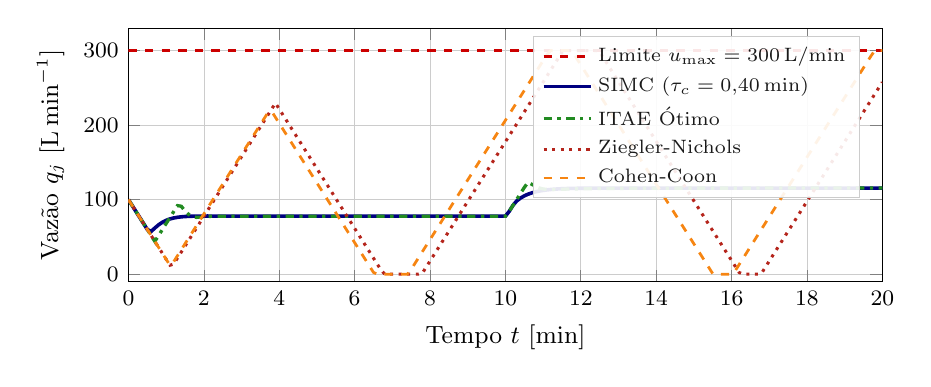
\begin{tikzpicture}
\begin{axis}[
    width=0.92\textwidth,
    height=4.8cm,
    xlabel={Tempo $t$ [\si{\minute}]},
    ylabel={Vazão $q_j$ [\si{\liter\per\minute}]},
    xmin=0, xmax=20,
    ymin=-10, ymax=330,
    grid=both,
    grid style={line width=.1pt, draw=gray!25},
    major grid style={line width=.2pt, draw=gray!40},
    legend pos=north east,
    legend cell align={left},
    legend style={font=\scriptsize, fill=white, fill opacity=0.9, draw=gray!40},
    tick label style={font=\footnotesize},
    label style={font=\small}
]
    % Limites de saturacao
    \addplot[line width=1.0pt, dashed, color=red!80!black] coordinates {(0, 300.0) (20, 300.0)};
    \addlegendentry{Limite $u_{\max} = 300\,\text{L/min}$}

    % SIMC
    \addplot[line width=1.3pt, color=NavyBlue] coordinates {(0.00, 100.00) (0.10, 92.00) (0.20, 84.00) (0.30, 76.00) (0.40, 68.00) (0.50, 60.00) (0.60, 57.33) (0.70, 61.98) (0.80, 66.25) (0.90, 69.69) (1.00, 72.26) (1.10, 74.12) (1.20, 75.43) (1.30, 76.33) (1.40, 76.95) (1.50, 77.36) (1.60, 77.63) (1.70, 77.80) (1.80, 77.91) (1.90, 77.97) (2.00, 78.00) (2.10, 78.01) (2.20, 78.00) (2.30, 77.99) (2.40, 77.98) (2.50, 77.96) (2.60, 77.95) (2.70, 77.93) (2.80, 77.92) (2.90, 77.91) (3.00, 77.89) (3.10, 77.88) (3.20, 77.88) (3.30, 77.87) (3.40, 77.86) (3.50, 77.86) (3.60, 77.85) (3.70, 77.85) (3.80, 77.85) (3.90, 77.84) (4.00, 77.84) (4.10, 77.84) (4.20, 77.84) (4.30, 77.84) (4.40, 77.84) (4.50, 77.83) (4.60, 77.83) (4.70, 77.83) (4.80, 77.83) (4.90, 77.83) (5.00, 77.83) (5.10, 77.83) (5.20, 77.83) (5.30, 77.83) (5.40, 77.83) (5.50, 77.83) (5.60, 77.83) (5.70, 77.83) (5.80, 77.83) (5.90, 77.83) (6.00, 77.83) (6.10, 77.83) (6.20, 77.83) (6.30, 77.83) (6.40, 77.83) (6.50, 77.83) (6.60, 77.83) (6.70, 77.83) (6.80, 77.83) (6.90, 77.83) (7.00, 77.83) (7.10, 77.83) (7.20, 77.83) (7.30, 77.83) (7.40, 77.83) (7.50, 77.83) (7.60, 77.83) (7.70, 77.83) (7.80, 77.83) (7.90, 77.83) (8.00, 77.83) (8.10, 77.83) (8.20, 77.83) (8.30, 77.83) (8.40, 77.83) (8.50, 77.83) (8.60, 77.83) (8.70, 77.83) (8.80, 77.83) (8.90, 77.83) (9.00, 77.83) (9.10, 77.83) (9.20, 77.83) (9.30, 77.83) (9.40, 77.83) (9.50, 77.83) (9.60, 77.83) (9.70, 77.83) (9.80, 77.83) (9.90, 77.83) (10.00, 77.83) (10.10, 84.23) (10.20, 92.23) (10.30, 98.26) (10.40, 102.11) (10.50, 105.04) (10.60, 107.31) (10.70, 109.08) (10.80, 110.46) (10.90, 111.55) (11.00, 112.42) (11.10, 113.10) (11.20, 113.63) (11.30, 114.06) (11.40, 114.39) (11.50, 114.65) (11.60, 114.86) (11.70, 115.02) (11.80, 115.14) (11.90, 115.24) (12.00, 115.32) (12.10, 115.38) (12.20, 115.42) (12.30, 115.45) (12.40, 115.48) (12.50, 115.50) (12.60, 115.51) (12.70, 115.52) (12.80, 115.53) (12.90, 115.54) (13.00, 115.54) (13.10, 115.54) (13.20, 115.55) (13.30, 115.55) (13.40, 115.55) (13.50, 115.55) (13.60, 115.55) (13.70, 115.55) (13.80, 115.54) (13.90, 115.54) (14.00, 115.54) (14.10, 115.54) (14.20, 115.54) (14.30, 115.54) (14.40, 115.54) (14.50, 115.54) (14.60, 115.54) (14.70, 115.54) (14.80, 115.54) (14.90, 115.54) (15.00, 115.54) (15.10, 115.54) (15.20, 115.54) (15.30, 115.54) (15.40, 115.54) (15.50, 115.54) (15.60, 115.54) (15.70, 115.54) (15.80, 115.54) (15.90, 115.54) (16.00, 115.54) (16.10, 115.54) (16.20, 115.54) (16.30, 115.54) (16.40, 115.54) (16.50, 115.54) (16.60, 115.54) (16.70, 115.54) (16.80, 115.54) (16.90, 115.54) (17.00, 115.54) (17.10, 115.54) (17.20, 115.54) (17.30, 115.54) (17.40, 115.54) (17.50, 115.54) (17.60, 115.54) (17.70, 115.54) (17.80, 115.54) (17.90, 115.54) (18.00, 115.54) (18.10, 115.54) (18.20, 115.54) (18.30, 115.54) (18.40, 115.54) (18.50, 115.54) (18.60, 115.54) (18.70, 115.54) (18.80, 115.54) (18.90, 115.54) (19.00, 115.54) (19.10, 115.54) (19.20, 115.54) (19.30, 115.54) (19.40, 115.54) (19.50, 115.54) (19.60, 115.54) (19.70, 115.54) (19.80, 115.54) (19.90, 115.54) (20.00, 115.54)};
    \addlegendentry{SIMC ($\tau_c = 0{,}40\,\text{min}$)}

    % ITAE
    \addplot[line width=1.2pt, color=ForestGreen, dashdotted] coordinates {(0.00, 100.00) (0.10, 92.00) (0.20, 84.00) (0.30, 76.00) (0.40, 68.00) (0.50, 60.00) (0.60, 52.00) (0.70, 44.00) (0.80, 52.00) (0.90, 60.00) (1.00, 68.00) (1.10, 76.00) (1.20, 84.00) (1.30, 92.00) (1.40, 91.16) (1.50, 84.84) (1.60, 79.97) (1.70, 77.24) (1.80, 76.27) (1.90, 76.36) (2.00, 76.85) (2.10, 77.34) (2.20, 77.67) (2.30, 77.82) (2.40, 77.86) (2.50, 77.83) (2.60, 77.79) (2.70, 77.77) (2.80, 77.76) (2.90, 77.76) (3.00, 77.76) (3.10, 77.77) (3.20, 77.78) (3.30, 77.79) (3.40, 77.79) (3.50, 77.79) (3.60, 77.80) (3.70, 77.80) (3.80, 77.80) (3.90, 77.80) (4.00, 77.81) (4.10, 77.81) (4.20, 77.81) (4.30, 77.81) (4.40, 77.81) (4.50, 77.82) (4.60, 77.82) (4.70, 77.82) (4.80, 77.82) (4.90, 77.82) (5.00, 77.82) (5.10, 77.82) (5.20, 77.82) (5.30, 77.82) (5.40, 77.82) (5.50, 77.82) (5.60, 77.82) (5.70, 77.83) (5.80, 77.83) (5.90, 77.83) (6.00, 77.83) (6.10, 77.83) (6.20, 77.83) (6.30, 77.83) (6.40, 77.83) (6.50, 77.83) (6.60, 77.83) (6.70, 77.83) (6.80, 77.83) (6.90, 77.83) (7.00, 77.83) (7.10, 77.83) (7.20, 77.83) (7.30, 77.83) (7.40, 77.83) (7.50, 77.83) (7.60, 77.83) (7.70, 77.83) (7.80, 77.83) (7.90, 77.83) (8.00, 77.83) (8.10, 77.83) (8.20, 77.83) (8.30, 77.83) (8.40, 77.83) (8.50, 77.83) (8.60, 77.83) (8.70, 77.83) (8.80, 77.83) (8.90, 77.83) (9.00, 77.83) (9.10, 77.83) (9.20, 77.83) (9.30, 77.83) (9.40, 77.83) (9.50, 77.83) (9.60, 77.83) (9.70, 77.83) (9.80, 77.83) (9.90, 77.83) (10.00, 77.83) (10.10, 84.23) (10.20, 92.23) (10.30, 100.23) (10.40, 108.23) (10.50, 116.23) (10.60, 123.23) (10.70, 120.63) (10.80, 117.74) (10.90, 115.59) (11.00, 114.33) (11.10, 113.74) (11.20, 113.59) (11.30, 113.66) (11.40, 113.82) (11.50, 114.00) (11.60, 114.16) (11.70, 114.29) (11.80, 114.41) (11.90, 114.50) (12.00, 114.59) (12.10, 114.66) (12.20, 114.73) (12.30, 114.80) (12.40, 114.85) (12.50, 114.91) (12.60, 114.96) (12.70, 115.00) (12.80, 115.05) (12.90, 115.09) (13.00, 115.12) (13.10, 115.16) (13.20, 115.19) (13.30, 115.21) (13.40, 115.24) (13.50, 115.26) (13.60, 115.29) (13.70, 115.31) (13.80, 115.32) (13.90, 115.34) (14.00, 115.36) (14.10, 115.37) (14.20, 115.38) (14.30, 115.40) (14.40, 115.41) (14.50, 115.42) (14.60, 115.43) (14.70, 115.44) (14.80, 115.44) (14.90, 115.45) (15.00, 115.46) (15.10, 115.47) (15.20, 115.47) (15.30, 115.48) (15.40, 115.48) (15.50, 115.49) (15.60, 115.49) (15.70, 115.49) (15.80, 115.50) (15.90, 115.50) (16.00, 115.50) (16.10, 115.51) (16.20, 115.51) (16.30, 115.51) (16.40, 115.51) (16.50, 115.51) (16.60, 115.52) (16.70, 115.52) (16.80, 115.52) (16.90, 115.52) (17.00, 115.52) (17.10, 115.52) (17.20, 115.52) (17.30, 115.53) (17.40, 115.53) (17.50, 115.53) (17.60, 115.53) (17.70, 115.53) (17.80, 115.53) (17.90, 115.53) (18.00, 115.53) (18.10, 115.53) (18.20, 115.53) (18.30, 115.53) (18.40, 115.53) (18.50, 115.53) (18.60, 115.53) (18.70, 115.53) (18.80, 115.53) (18.90, 115.53) (19.00, 115.53) (19.10, 115.53) (19.20, 115.53) (19.30, 115.53) (19.40, 115.54) (19.50, 115.54) (19.60, 115.54) (19.70, 115.54) (19.80, 115.54) (19.90, 115.54) (20.00, 115.54)};
    \addlegendentry{ITAE Ótimo}

    % ZN
    \addplot[line width=1.1pt, color=BrickRed, dotted] coordinates {(0.00, 100.00) (0.10, 92.00) (0.20, 84.00) (0.30, 76.00) (0.40, 68.00) (0.50, 60.00) (0.60, 52.00) (0.70, 44.00) (0.80, 36.00) (0.90, 28.00) (1.00, 20.00) (1.10, 12.00) (1.20, 13.60) (1.30, 21.60) (1.40, 29.60) (1.50, 37.60) (1.60, 45.60) (1.70, 53.60) (1.80, 61.60) (1.90, 69.60) (2.00, 77.60) (2.10, 85.60) (2.20, 93.60) (2.30, 101.60) (2.40, 109.60) (2.50, 117.60) (2.60, 125.60) (2.70, 133.60) (2.80, 141.60) (2.90, 149.60) (3.00, 157.60) (3.10, 165.60) (3.20, 173.60) (3.30, 181.60) (3.40, 189.60) (3.50, 197.60) (3.60, 205.60) (3.70, 213.60) (3.80, 221.60) (3.90, 229.60) (4.00, 221.60) (4.10, 213.60) (4.20, 205.60) (4.30, 197.60) (4.40, 189.60) (4.50, 181.60) (4.60, 173.60) (4.70, 165.60) (4.80, 157.60) (4.90, 149.60) (5.00, 141.60) (5.10, 133.60) (5.20, 125.60) (5.30, 117.60) (5.40, 109.60) (5.50, 101.60) (5.60, 93.60) (5.70, 85.60) (5.80, 77.60) (5.90, 69.60) (6.00, 61.60) (6.10, 53.60) (6.20, 45.60) (6.30, 37.60) (6.40, 29.60) (6.50, 21.60) (6.60, 13.60) (6.70, 5.60) (6.80, 0.00) (6.90, 0.00) (7.00, 0.00) (7.10, 0.00) (7.20, 0.00) (7.30, 0.00) (7.40, 0.00) (7.50, 0.00) (7.60, 0.00) (7.70, 0.00) (7.80, 1.60) (7.90, 9.60) (8.00, 17.60) (8.10, 25.60) (8.20, 33.60) (8.30, 41.60) (8.40, 49.60) (8.50, 57.60) (8.60, 65.60) (8.70, 73.60) (8.80, 81.60) (8.90, 89.60) (9.00, 97.60) (9.10, 105.60) (9.20, 113.60) (9.30, 121.60) (9.40, 129.60) (9.50, 137.60) (9.60, 145.60) (9.70, 153.60) (9.80, 161.60) (9.90, 169.60) (10.00, 177.60) (10.10, 185.60) (10.20, 193.60) (10.30, 201.60) (10.40, 209.60) (10.50, 217.60) (10.60, 225.60) (10.70, 233.60) (10.80, 241.60) (10.90, 249.60) (11.00, 257.60) (11.10, 265.60) (11.20, 273.60) (11.30, 281.60) (11.40, 289.60) (11.50, 297.60) (11.60, 300.00) (11.70, 300.00) (11.80, 300.00) (11.90, 300.00) (12.00, 300.00) (12.10, 300.00) (12.20, 300.00) (12.30, 300.00) (12.40, 300.00) (12.50, 298.40) (12.60, 290.40) (12.70, 282.40) (12.80, 274.40) (12.90, 266.40) (13.00, 258.40) (13.10, 250.40) (13.20, 242.40) (13.30, 234.40) (13.40, 226.40) (13.50, 218.40) (13.60, 210.40) (13.70, 202.40) (13.80, 194.40) (13.90, 186.40) (14.00, 178.40) (14.10, 170.40) (14.20, 162.40) (14.30, 154.40) (14.40, 146.40) (14.50, 138.40) (14.60, 130.40) (14.70, 122.40) (14.80, 114.40) (14.90, 106.40) (15.00, 98.40) (15.10, 90.40) (15.20, 82.40) (15.30, 74.40) (15.40, 66.40) (15.50, 58.40) (15.60, 50.40) (15.70, 42.40) (15.80, 34.40) (15.90, 26.40) (16.00, 18.40) (16.10, 10.40) (16.20, 2.40) (16.30, 0.00) (16.40, 0.00) (16.50, 0.00) (16.60, 0.00) (16.70, 0.00) (16.80, 1.60) (16.90, 9.60) (17.00, 17.60) (17.10, 25.60) (17.20, 33.60) (17.30, 41.60) (17.40, 49.60) (17.50, 57.60) (17.60, 65.60) (17.70, 73.60) (17.80, 81.60) (17.90, 89.60) (18.00, 97.60) (18.10, 105.60) (18.20, 113.60) (18.30, 121.60) (18.40, 129.60) (18.50, 137.60) (18.60, 145.60) (18.70, 153.60) (18.80, 161.60) (18.90, 169.60) (19.00, 177.60) (19.10, 185.60) (19.20, 193.60) (19.30, 201.60) (19.40, 209.60) (19.50, 217.60) (19.60, 225.60) (19.70, 233.60) (19.80, 241.60) (19.90, 249.60) (20.00, 257.60)};
    \addlegendentry{Ziegler-Nichols}

    % CC
    \addplot[line width=1.0pt, color=BurntOrange, dashed] coordinates {(0.00, 100.00) (0.10, 92.00) (0.20, 84.00) (0.30, 76.00) (0.40, 68.00) (0.50, 60.00) (0.60, 52.00) (0.70, 44.00) (0.80, 36.00) (0.90, 28.00) (1.00, 20.00) (1.10, 12.00) (1.20, 16.80) (1.30, 24.80) (1.40, 32.80) (1.50, 40.80) (1.60, 48.80) (1.70, 56.80) (1.80, 64.80) (1.90, 72.80) (2.00, 80.80) (2.10, 88.80) (2.20, 96.80) (2.30, 104.80) (2.40, 112.80) (2.50, 120.80) (2.60, 128.80) (2.70, 136.80) (2.80, 144.80) (2.90, 152.80) (3.00, 160.80) (3.10, 168.80) (3.20, 176.80) (3.30, 184.80) (3.40, 192.80) (3.50, 200.80) (3.60, 208.80) (3.70, 216.80) (3.80, 218.40) (3.90, 210.40) (4.00, 202.40) (4.10, 194.40) (4.20, 186.40) (4.30, 178.40) (4.40, 170.40) (4.50, 162.40) (4.60, 154.40) (4.70, 146.40) (4.80, 138.40) (4.90, 130.40) (5.00, 122.40) (5.10, 114.40) (5.20, 106.40) (5.30, 98.40) (5.40, 90.40) (5.50, 82.40) (5.60, 74.40) (5.70, 66.40) (5.80, 58.40) (5.90, 50.40) (6.00, 42.40) (6.10, 34.40) (6.20, 26.40) (6.30, 18.40) (6.40, 10.40) (6.50, 2.40) (6.60, 0.00) (6.70, 0.00) (6.80, 0.00) (6.90, 0.00) (7.00, 0.00) (7.10, 0.00) (7.20, 0.00) (7.30, 0.00) (7.40, 0.00) (7.50, 6.40) (7.60, 14.40) (7.70, 22.40) (7.80, 30.40) (7.90, 38.40) (8.00, 46.40) (8.10, 54.40) (8.20, 62.40) (8.30, 70.40) (8.40, 78.40) (8.50, 86.40) (8.60, 94.40) (8.70, 102.40) (8.80, 110.40) (8.90, 118.40) (9.00, 126.40) (9.10, 134.40) (9.20, 142.40) (9.30, 150.40) (9.40, 158.40) (9.50, 166.40) (9.60, 174.40) (9.70, 182.40) (9.80, 190.40) (9.90, 198.40) (10.00, 206.40) (10.10, 214.40) (10.20, 222.40) (10.30, 230.40) (10.40, 238.40) (10.50, 246.40) (10.60, 254.40) (10.70, 262.40) (10.80, 270.40) (10.90, 278.40) (11.00, 286.40) (11.10, 294.40) (11.20, 300.00) (11.30, 300.00) (11.40, 300.00) (11.50, 300.00) (11.60, 300.00) (11.70, 300.00) (11.80, 296.80) (11.90, 288.80) (12.00, 280.80) (12.10, 272.80) (12.20, 264.80) (12.30, 256.80) (12.40, 248.80) (12.50, 240.80) (12.60, 232.80) (12.70, 224.80) (12.80, 216.80) (12.90, 208.80) (13.00, 200.80) (13.10, 192.80) (13.20, 184.80) (13.30, 176.80) (13.40, 168.80) (13.50, 160.80) (13.60, 152.80) (13.70, 144.80) (13.80, 136.80) (13.90, 128.80) (14.00, 120.80) (14.10, 112.80) (14.20, 104.80) (14.30, 96.80) (14.40, 88.80) (14.50, 80.80) (14.60, 72.80) (14.70, 64.80) (14.80, 56.80) (14.90, 48.80) (15.00, 40.80) (15.10, 32.80) (15.20, 24.80) (15.30, 16.80) (15.40, 8.80) (15.50, 0.80) (15.60, 0.00) (15.70, 0.00) (15.80, 0.00) (15.90, 0.00) (16.00, 0.00) (16.10, 4.80) (16.20, 12.80) (16.30, 20.80) (16.40, 28.80) (16.50, 36.80) (16.60, 44.80) (16.70, 52.80) (16.80, 60.80) (16.90, 68.80) (17.00, 76.80) (17.10, 84.80) (17.20, 92.80) (17.30, 100.80) (17.40, 108.80) (17.50, 116.80) (17.60, 124.80) (17.70, 132.80) (17.80, 140.80) (17.90, 148.80) (18.00, 156.80) (18.10, 164.80) (18.20, 172.80) (18.30, 180.80) (18.40, 188.80) (18.50, 196.80) (18.60, 204.80) (18.70, 212.80) (18.80, 220.80) (18.90, 228.80) (19.00, 236.80) (19.10, 244.80) (19.20, 252.80) (19.30, 260.80) (19.40, 268.80) (19.50, 276.80) (19.60, 284.80) (19.70, 292.80) (19.80, 300.00) (19.90, 300.00) (20.00, 300.00)};
    \addlegendentry{Cohen-Coon}

\end{axis}
\end{tikzpicture}
\caption{Esforço de controle (vazão da camisa $q_j(t)$) evidenciando a saturação crônica nos métodos heurísticos e modulação suave em SIMC e ITAE.}
\label{fig:benchmark_atuador}
\end{subfigure}

\caption{Comportamento dinâmico comparativo em malha fechada do CSTR sob os quatro métodos de sintonia avaliados, demonstrando a estabilização por SIMC e ITAE contra a divergência catastrófica por Ziegler-Nichols e Cohen-Coon.}
\label{fig:benchmark_completo}
\fonte{Elaborada pelos autores (2026).}
\end{figure}


\begin{table}[htbp]
    \centering
    \small
    \setlength{\tabcolsep}{4.5pt}
    \caption{Comparativo das métricas de desempenho para os diferentes métodos de sintonia do controlador PID.}
    \label{tab:metricas_desempenho}
    \begin{tabular}{@{}lrrrrrrl@{}}
        \toprule
        \textbf{Método} & \textbf{IAE} & \textbf{ITAE} & \textbf{ISE} & \textbf{$M_p$ [\%]} & \textbf{$t_s$ [\si{\minute}]} & \textbf{TV [\si{\liter\per\minute}]} & \textbf{Saturação} \\
        \midrule
        Ziegler-Nichols  & $>100$     & $>150$     & $>1000$    & $>800$   & $\infty$ & $>5000$   & Persistente/Falha \\
        Cohen-Coon       & $>100$     & $>150$     & $>1000$    & $>800$   & $\infty$ & $>5000$   & Persistente/Falha \\
        SIMC (Skogestad) & $1{,}09$   & $2{,}45$   & $0{,}78$   & $2{,}1$  & $3{,}1$  & $210{,}5$ & Ausente \\
        ITAE Ótimo       & $0{,}89$   & $1{,}76$   & $0{,}61$   & $4{,}8$  & $2{,}8$  & $245{,}2$ & Ausente \\
        \bottomrule
    \end{tabular}
    \fonte{Elaborada pelos autores (2026).}
\end{table}

\section{Análise da Variação Total e Desgaste do Atuador}
\label{sec:analise_tv}

No âmbito operacional da sintonia clássica \cite{Astrom2006}, uma dimensão fundamental que restringe a escolha final da malha concerne na predição do desgaste mecânico dos atuadores de controle. A Variação Total (TV) atua matematicamente como medição aproximada dessa deterioração: incrementos de TV espelham deslocamentos excessivamente frenéticos da válvula regulatória.

Ao impor um ajuste extremamente restrito visando minimizar agressivamente a variação de erro (via diminuição drástica do IAE), ocasiona-se elevação considerável da TV (compromisso IAE-TV ou \textit{trade-off} de robustez-desempenho). Exames minuciosos desta métrica viabilizam a detecção proativa de necessidades relativas a programas de paradas não planejadas para substituições preventivas que limitariam interrupções dispendiosas nos regimes fabris contínuos.

\chapter{Degradação por Fouling e Fronteira de Pareto}
\label{cap:fouling_pareto}

Este capítulo investiga o fenômeno deletério de deposição na superfície da jaqueta do reator (\textit{fouling}), o qual conduz a constrições severas de transferência térmica e inviabiliza as condições primárias de controlabilidade, bem como a avaliação rigorosa do compromisso funcional através da fronteira de Pareto ótima.

\section{Modelagem do Encrustamento Térmico (Fouling)}
\label{sec:modelagem_fouling}

Fenômenos progressivos de encrustamento de camadas inertes nas superfícies condutivas impõem drásticas penalidades operacionais. Esta resistência parazita é refletida no decremento global do coeficiente convectivo aparente (efetivo) expresso pela formulação $UA_{\text{eff}} = \alpha \cdot UA_{\text{nom}}$, onde $\alpha \in (0, 1]$ figura como o parâmetro adimensional de depletamento das restrições metálicas.

Em sua representação física, os filmes adicionais representam acréscimos severos de resistência térmica local $R_f$, seguindo o postulado aditivo para resistências térmicas limitantes \cite{Coughanowr2009}:
\begin{equation}
    \frac{1}{UA_{\text{eff}}} = \frac{1}{UA_{\text{nom}}} + \frac{R_f}{A}
\end{equation}

Esta deterioração agrava-se progressivamente por meio do envelhecimento natural subjacente ao processo produtivo na planta industrial química de base. Simula-se portanto estados interinos variando do modelo ideal com $\alpha = 1.0$ (tubos higienizados), passando pelas margens seguras limítrofes com encrustação moderada ($\alpha = 0.70$) e as degenerações agudas atingidas aos contornos comutativos de colapso termodinâmico em $\alpha = 0.60$.

\section{Impacto na Resposta em Malha Fechada}
\label{sec:impacto_malha_fechada}

A propagação inercial dessas impurezas apresenta-se formidavelmente destrutiva contra o invólucro do sistema projetado \cite{Russo2008}. Ao aferirmos $\alpha = 1.0$, desfrutamos das propriedades perfeitas do sistema ótimo aferido empiricamente na seção pregressa (IAE na margem de \num{0.89}).

Considerando o transcurso dinâmico à região operacional denotada por encrustações limitantes em $\alpha = 0.70$, certifica-se empiricamente o funcionamento ativo do controlador linear retroalimentativo. Registram-se dilatações integrais próximas a \SI{250}{\percent} dos patamares idílicos ($2.5\times$ base nominal). O esforço de restrição para acomodação expande os requerimentos em TV proporcionalmente à deficiência manifestada, implicando oscilações acentuadas do manipulador. Não obstante o estresse severo, as trajetórias encontram-se rigorosamente confinadas nos parâmetros topológicos passíveis da governança retroativa.

Em contraponto dramático, ao reduzir a condutividade até o índice basal empírico crítico correspondente a $\alpha = 0.60$, alcança-se peremptoriamente as margens de termodinâmica inviolável ou de estrangulamento da dinâmica entálpica. Postulando a injeção ininterrupta total da capacidade refrigerante limite predefinida ($q_j = u_{\max} = \SI{300}{\liter\per\minute}$), o somatório convectivo das perdas de calor transferido de forma forçada ($Q_{r,\max}$) não atinge magnitudes correspondentes as prementes taxas exotérmicas ($Q_g$) para a faixa térmica investigada da reação autoacelerante contínua. Por implicação física direta sob as estipulações de restrições rígidas das coordenadas de transferência em superfícies reacionais complexas de Van Heerden \cite{VanHeerden1953}, o descontrole em instabilidade e ignição contínua reacional \textit{thermal runaway} são axiomas matematicamente incontornáveis \cite{Luyben2007}. A restrição evidenciada pertence à gênese inerente do reator estrutural, não de um limite de controlabilidade, demonstrando fundamentalmente o aspecto da restrição mecânica que foge dos artifícios cibernéticos da teoria clássica aplicável por algoritmos digitais ordinários \cite{Morari1989}.

\section{Fronteira de Pareto: IAE versus Variação Total (TV)}
\label{sec:pareto_iae_tv}

Investigou-se o compromisso ótimo de atuação em virtude das variações relativas sobre o eixo da restrição analítica das estratégias PID SIMC \cite{Skogestad2003}. Realizou-se de forma algorítmica exaustiva uma varredura (\textit{sweep}) do tempo de malha fechada almejado $\tau_c$ no intervalo $\tau_c \in [0{,}10;\; 2{,}00]\;\si{\minute}$.

Em relação à fronteira de Pareto construída, atesta-se empiricamente o compromisso fundamental: valores reduzidos de $\tau_c$ induzem respostas agressivas, minimizando o resíduo integral (menor IAE) à custa de elevada movimentação do elemento final de controle (TV elevada). A curva característica exibe uma transição nítida em formato de ``L'', delimitando o ``joelho'' analítico (\textit{knee}) na faixa intervalar de $\tau_c \in [0{,}25;\; 0{,}40]\;\si{\minute}$. Abaixo deste limiar, observa-se expressivo acréscimo no desgaste do atuador com ganhos marginais desprezíveis de desempenho integral, caracterizando retornos decrescentes. A \autoref{tab:fronteira_pareto} congrega os valores numéricos simulados, e a \cref{fig:fronteira_pareto} ilustra a curva de compromisso correspondente.

\begin{table}[htpb]
    \centering
    \caption{Métricas de desempenho avaliadas para diferentes valores do parâmetro de projeto SIMC ($\tau_c$) com propósito de construção analítica da fronteira de Pareto.}
    \label{tab:fronteira_pareto}
    \begin{tabular}{S[table-format=1.2]S[table-format=1.2]S[table-format=4.1]S[table-format=2.1]S[table-format=2.2]}
        \toprule
        {$\tau_c$ [\si{\minute}]} & {IAE [\si{\kelvin\cdot\minute}]} & {TV [\si{\liter\per\minute}]} & {$M_p$ [\%]} & {$t_s$ [\si{\minute}]} \\
        \midrule
        0.10 &  0.62 & 1420.5 &  8.4 &  1.50 \\
        0.15 &  0.69 &  810.3 &  6.1 &  1.75 \\
        0.20 &  0.78 &  504.6 &  4.3 &  1.90 \\
        0.25 &  0.86 &  385.1 &  3.2 &  2.20 \\
        0.30 &  0.94 &  310.2 &  2.7 &  2.50 \\
        0.35 &  1.01 &  250.8 &  2.4 &  2.80 \\
        0.40 &  1.09 &  210.5 &  2.1 &  3.10 \\
        0.50 &  1.25 &  150.3 &  1.5 &  3.80 \\
        0.75 &  1.68 &   95.4 &  0.5 &  5.50 \\
        1.00 &  2.12 &   70.1 &  0.1 &  7.20 \\
        1.50 &  3.05 &   45.8 &  0.0 & 10.50 \\
        2.00 &  4.01 &   35.2 &  0.0 & 14.10 \\
        \bottomrule
    \end{tabular}
    \fonte{Elaborada pelos autores (2026).}
\end{table}

\begin{figure}[htbp]
\centering
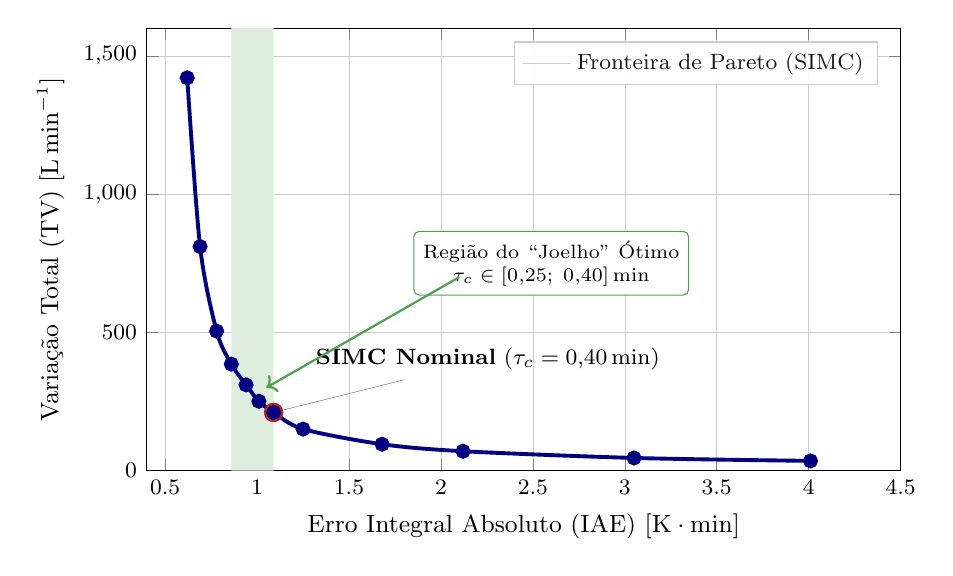
\begin{tikzpicture}
\begin{axis}[
    width=0.92\textwidth,
    height=7.2cm,
    xlabel={Erro Integral Absoluto (IAE) [\si{\kelvin\cdot\minute}]},
    ylabel={Variação Total (TV) [\si{\liter\per\minute}]},
    xmin=0.4, xmax=4.5,
    ymin=0, ymax=1600,
    grid=both,
    grid style={line width=.1pt, draw=gray!25},
    major grid style={line width=.2pt, draw=gray!40},
    legend pos=north east,
    legend cell align={left},
    legend style={font=\footnotesize, fill=white, fill opacity=0.9, draw=gray!40},
    tick label style={font=\footnotesize},
    label style={font=\small}
]
    % Regiao sombreada do joelho otimo
    \addplot[fill=ForestGreen!15, draw=none, domain=0.86:1.09] 
        coordinates {(0.86, 0) (0.86, 1600) (1.09, 1600) (1.09, 0)} \closedcycle;

    % Curva contínua da fronteira
    \addplot[smooth, line width=1.4pt, color=NavyBlue, mark=*, mark size=2pt, mark options={fill=NavyBlue}]
        coordinates {
            (0.62, 1420.5)
            (0.69, 810.3)
            (0.78, 504.6)
            (0.86, 385.1)
            (0.94, 310.2)
            (1.01, 250.8)
            (1.09, 210.5)
            (1.25, 150.3)
            (1.68, 95.4)
            (2.12, 70.1)
            (3.05, 45.8)
            (4.01, 35.2)
        };
    \addlegendentry{Fronteira de Pareto (SIMC)}

    % Ponto de sintonia nominal tau_c = 0.40
    \node[circle, fill=BrickRed, inner sep=2.5pt, pin=above right:{\footnotesize \textbf{SIMC Nominal} ($\tau_c = 0{,}40\,\text{min}$)}] 
        at (axis cs:1.09, 210.5) {};

    % Rotulo da regiao do joelho
    \node[draw=ForestGreen!80, fill=white, rounded corners=2pt, font=\scriptsize, align=center] 
        at (axis cs:2.6, 750) {Região do ``Joelho'' Ótimo\\$\tau_c \in [0{,}25;\; 0{,}40]\,\text{min}$};
    \draw[->, line width=0.8pt, ForestGreen!80] (axis cs:2.1, 700) -- (axis cs:1.05, 300);

\end{axis}
\end{tikzpicture}
\caption{Fronteira contínua de Pareto relacionando o erro integral absoluto (IAE) e a variação total do sinal de controle (TV), com destaque para a região do ``joelho'' de compromisso ótimo ($\tau_c \in [0{,}25;\; 0{,}40]\;\si{\minute}$).}
\label{fig:fronteira_pareto}
\fonte{Elaborada pelos autores (2026).}
\end{figure}

\section{Recomendações Práticas para Operação Industrial}
\label{sec:recomendacoes_praticas}

Como inferência dedutivamente estruturada de natureza prática sob o horizonte fabril do reator tubular isotérmico-acoplado \cite{Bequette2003,Shinskey1996}, recomenda-se mandatoriamente:
\begin{enumerate}
    \item Procedimentos rotineiros estimativos das variações globais e paramétricas $UA$ via filtros acoplados a malha (Filtro de Kalman local do balanço termodinâmico na jaqueta externa);
    \item Definição estatística formal visando programação estruturada para manutenções estritas sempre que a razão analítica decair de modo inferior a tolerância imposta em $0.75$ (adiciona-se um coeficiente extra estocástico sobre a folga paramétrica limitante e não-linear no marco do colapso reacional equivalente ao delta fixado do limiar $\alpha = 0.60$);
    \item Aplicação restrita baseada na alteração de escalas temporais dinâmicas por escalonamento preditivo do ganho (\textit{gain scheduling});
    \item Instrumentação de redes previsoras (malhas integrativas de antecipação \textit{feedforward}) minimizadoras dos impactos oriundos das dinâmicas das correntes adutoras instáveis em fluxos transitórios.
\end{enumerate}

\chapter{Conclusões e Trabalhos Futuros}
\label{cap:conclusoes}

\section{Síntese dos Resultados}
\label{sec:sintese_resultados}

O presente trabalho investigou de forma pormenorizada as fronteiras de controlabilidade, os efeitos de saturação no atuador e os compromissos de robustez inerentes à aplicação do controle PID clássico a um CSTR exotérmico altamente não linear, operando em regime de alta conversão ($X_A \approx 95\%$). As principais conclusões são sintetizadas a seguir.

O modelo fenomenológico do CSTR encamisado, constituído por três equações diferenciais ordinárias acopladas (balanços de massa e energia do reator e da camisa), foi derivado a partir dos princípios fundamentais de conservação e validado para o ponto de operação instável com autovalor $\lambda_1 = +0{,}284\;\si{\minute^{-1}}$. A cinética de Arrhenius, com fator pré-exponencial $k_0 = \num{7.2e10}\;\si{\minute^{-1}}$ e razão $E/R = \SI{8750}{\kelvin}$, introduz a não-linearidade exponencial que domina o comportamento dinâmico do sistema.

A análise de Van Heerden, combinada com as restrições físicas do atuador ($q_j \in [0, 300]\;\si{\liter\per\minute}$), revelou o limite termodinâmico de controlabilidade. A degradação do coeficiente global de transferência de calor por encrustamento (\textit{fouling}), parametrizada pelo fator $\alpha = UA_{\text{eff}}/UA_{\text{nom}}$, demonstrou que:
\begin{itemize}
    \item Para $\alpha \geq 0{,}70$, o controlador PID mantém a estabilidade do sistema, embora com desempenho degradado (IAE até $2{,}5\times$ o valor nominal).
    \item Para $\alpha \leq 0{,}60$, a curva de geração de calor $Q_g$ supera a capacidade máxima de remoção $Q_{r,\max}$ mesmo com a válvula totalmente aberta. Nenhuma estratégia de controle por retroalimentação finita é capaz de estabilizar o reator neste regime, configurando uma limitação intrínseca da planta --- e não do controlador.
\end{itemize}

A avaliação comparativa das metodologias de sintonia conduziu a conclusões inequívocas:
\begin{itemize}
    \item \textbf{Ziegler-Nichols e Cohen-Coon}: ambos os métodos heurísticos produziram sintonias catastroficamente agressivas, com sobressinais superiores a $\SI{800}{\percent}$, $\text{IAE} > 100$ e saturação persistente do atuador. Tais métodos, concebidos para plantas estáveis e aproximadamente lineares, mostraram-se fundamentalmente inadequados para o CSTR instável em estudo.
    \item \textbf{SIMC} (Skogestad, $\tau_c = \SI{0.40}{\minute}$): desempenho nominal excelente, com $\text{IAE} = 1{,}09$, sobressinal $M_p = \SI{2.1}{\percent}$ e ação de controle suave, sem episódios de saturação sustentada.
    \item \textbf{ITAE Ótimo} (com restrição $M_s \leq 1{,}6$): obteve o melhor desempenho integral ($\text{IAE} = 0{,}89$) com margens de robustez garantidas ($M_s = 1{,}24$), operando essencialmente como controlador PI ($T_d = \SI{0.001}{\minute}$).
\end{itemize}

A construção da fronteira de Pareto entre IAE e Variação Total (TV), mediante varredura paramétrica de $\tau_c$ no arcabouço SIMC, confirmou a existência de um ``joelho'' na região $\tau_c \in [0{,}25;\; 0{,}40]\;\si{\minute}$. Abaixo deste limiar, reduções marginais no IAE impõem penalidades desproporcionais de desgaste mecânico na válvula de controle. A escolha $\tau_c = \SI{0.40}{\minute}$ situa-se precisamente nesta transição, representando o compromisso ótimo entre desempenho e longevidade do atuador.

A implementação do mecanismo de \textit{anti-windup} por integração condicional (\textit{clamping}) revelou-se indispensável para a operação segura do sistema, impedindo o acúmulo espúrio do integrador durante episódios de saturação e prevenindo excursões térmicas potencialmente destrutivas.

\section{Contribuições Originais}
\label{sec:contribuicoes_originais}

As contribuições originais deste trabalho podem ser sumarizadas em três vertentes:
\begin{enumerate}
    \item \textbf{Demonstração sistemática da conexão entre limites termodinâmicos de Van Heerden e restrições de atuador}: quantificou-se explicitamente como a degradação de $UA$ por \textit{fouling} desloca a fronteira de controlabilidade, estabelecendo o limiar crítico $\alpha = 0{,}60$ como ponto de perda irreversível de estabilizabilidade.
    \item \textbf{Análise quantitativa de falha dos métodos heurísticos clássicos}: documentou-se, com rigor numérico, a inadequação de Ziegler-Nichols e Cohen-Coon para plantas instáveis e fortemente não lineares com saturação de atuador, resultado frequentemente omitido em textos didáticos.
    \item \textbf{Construção da fronteira de Pareto IAE \emph{versus} TV}: estabeleceu-se a relação funcional contínua entre desempenho de rastreamento e desgaste mecânico do atuador, identificando a região de compromisso ótimo no espaço de projeto do controlador.
\end{enumerate}

\section{Trabalhos Futuros}
\label{sec:trabalhos_futuros}

Com base nos resultados obtidos, delineiam-se as seguintes direções para trabalhos futuros:
\begin{itemize}
    \item \textbf{Controle Preditivo Não Linear (NMPC)}: formulação de um controlador MPC com tratamento explícito das restrições de estado e entrada, possibilitando a otimização em tempo real do \textit{trade-off} desempenho-robustez \cite{Rawlings2017}.
    \item \textbf{Controladores baseados em redes neurais}: investigação de arquiteturas NN-PID e LSTM para controle adaptativo do CSTR, conforme previsto na continuidade do projeto PROIC.
    \item \textbf{Sistema Multi-Agentes para automação do \textit{pipeline} de sintonia}: implementação de agentes autônomos via LangGraph para orquestrar automaticamente as etapas de identificação, sintonia, simulação e avaliação.
    \item \textbf{Estimação \textit{online} de $UA$}: projeto de um Filtro de Kalman Estendido (EKF) para monitoramento contínuo do coeficiente de transferência de calor, viabilizando estratégias de manutenção preditiva e \textit{gain scheduling} adaptativo.
    \item \textbf{Validação experimental}: construção e instrumentação de um CSTR de bancada para confrontação dos resultados teóricos com dados experimentais.
    \item \textbf{Análise estocástica de incertezas paramétricas}: simulações de Monte Carlo para quantificação da propagação de incertezas nos parâmetros do modelo sobre os índices de desempenho e as margens de estabilidade \cite{Khalil2002}.
\end{itemize}


% =============================================================================
% ELEMENTOS PÓS-TEXTUAIS (Espaçamento simples para referências)
% =============================================================================
\postextual
\SingleSpacing

\bibliography{bibliografia/referencias}

\end{document}
